\documentclass[11pt]{report}
\usepackage{graphics}
\usepackage{graphicx}
\usepackage{epsfig}
\usepackage{fancyhdr}
%\usepackage{fullpage}
\usepackage{float}
\usepackage{xspace}
%\usepackage{algorithm}
%\usepackage{algorithmic}
%\usepackage{algorithmicx}

\begin{document}
\renewcommand\bibname{References}
\pagestyle{fancy}
%\fancyheadz{}
\fancyfoot{}
\fancyfoot[c]{\thepage}
\fancyfoot[l]{CSD334-Mini Project 2022}
\lhead{abcd}
\renewcommand{\chaptermark}[1]{
\markboth{\thechapter.\ #1}{}} 
\renewcommand{\headrulewidth}{0.1pt}
\fancyhead[r]{\slshape \leftmark}
\addtolength{\headheight}{\baselineskip}

\lhead{\nouppercase{\rightmark}}
\rhead{\nouppercase{\leftmark}}
%\lhead{hhhhh}
%\fancyhead[LO,RE]{\slshape \leftmark}
%\bibliographystyle{plain}
\title {E-Kart}
\author {Jaison Dennis}
%\maketitle

\begin{titlepage}
\begin{center}

%\topmargin100pt
\Huge{\textbf{E-MART}}\\
\large{\textbf{\\CSD334-Mini Project 2022\\}}
\vspace{1.2in}
\Large{\textbf{Jaison Dennis}}\\ 
\Large{\textbf{20CSA34\\
MDL20CS060\\
}}	\hspace{.1in}	

\Large{\textbf{
\\B. Tech. Computer Science \& Engineering
}}


\vspace{.6in}
\begin{figure}[h]
\begin{center}
%\epsfig{width=1in, file=embN1.jpg}

\epsfig{width=1in, file=logo.jpg}
% If you have access to better quality logo image, that may be used, but all the groups should use the same image
\end{center}
\end{figure}
%\vspace{.2in}
\textbf{
Department of Computer Engineering\\
Govt. Model Engineering College Thrikkakara\\
Thrikkakara, Kochi 682021\\
Phone: +91.484.2575370\\
http://www.mec.ac.in \\
hodcs@mec.ac.in
}
\end{center}
\end{titlepage}




\begin{titlepage}
\begin{center}
\Large{\textbf{Govt. Model Engineering College Thrikkakara}}\\
\Large{\textbf{\\Dept. of Computer Engineering}}\\
\end{center}
\begin{figure}[h]
\begin{center}

\epsfig{width=1in, file=logo.jpg}
\end{center}
\end{figure}
\begin{center}
\Large{\textbf{C E R T I F I C A T E}}\\
\vspace{.1in}
\end{center}
This is to certify that, this report titled \textbf{\textit {E-MART}} is a bonafide record of the work done by
{\textbf{20CSA34
MDL20CS060
}{\textbf{Jaison Dennis}}} {{, \textbf{Fifth Semester} B. Tech. Computer Science \& Engineering }}
student,  for the course work in \textbf{CSD334-Mini Project 2022} which is the Mini Project Work, under our guidance and supervision, in partial 
 fulfillment of the requirements for the award of the degree, B. Tech. Computer 
Science  and Engineering of \textbf{APJ Abdul Kalam University }.
\vspace{.1in}
\begin{tabbing}
xxxxxxxxxxxxxxxxxxxxxxxxxxxxxxxxxxxxxxxxxxxxxxx\= xxxxxxxxxxxxxxxxxx\= \kill

						Coordinator	\>Head of the Department
\\
\\
\\
  Veena Briji Philip\>Dr.Preetha Theresa Joy\\
	Assistant Professor\>Head of the Department
	
	 \\
	 \>Professor\\
Computer Engineering	\>	Computer Engineering
\end{tabbing}
\vspace{.08in}
%
\begin{tabbing}
xxxxxxxxxxxxxxxxxxxxxxxxxxxx\= xxxxxxxxxxxxxxxxxx\= \kill
			 \\
\\
\\
\today
\end{tabbing}
\end{titlepage}

\begin{center}
	\thispagestyle{empty}
	\LARGE{\textbf{Acknowledgements}}\\[1cm]
\end{center}
\linespread{1.13}
\large{\paragraph{}We would like to express deepest appreciation towards \textbf{Dr.Jacob Thomas},
	Principal, Govt. Model Enginnering College , Thrikkakara, \textbf{Prof. Preetha Theresa Joy}, 
	Head of Department of Computer Engineering and \textbf{Mrs.Veena Briji Philip }, Project Coordinator whose
	invaluable guidance supported us in completing this project.}
\large{\paragraph{}At last we must express our sincere heartfelt gratitude to all the staff members
	of Computer Engineering Department who helped me directly or indirectly during this course of work.}
\begin{flushright}
	{
		Jaison Dennis\\
		Jagannath E Shahi\\
		Christopher Roy
	}
\end{flushright}
\newpage
 
\begin{abstract}
\pagenumbering{roman}
This project 'E-Mart' is an e-commerce platform  which sells its goods and services online making it easier for the user to access a wide variety of items from a single platform. E-Mart allows customers to browse and purchase products from a variety of sellers through a web browser. The platform handles all aspects of the transaction, including payment processing, order fulfillment, and order tracking. The platform may also offer features such as personalized recommendations, wish lists, and reviews to help customers find the products they are looking for. Users can also add products to cart and buy them at a later time. Users can search and filter products based on price, brand and offers. Our platform is open for both end users and sellers. The goal of the platform is to create a convenient and easy-to-use shopping experience for customers, while also providing a means for sellers to reach a larger audience and grow their businesses.
\end{abstract}

\tableofcontents





\chapter {Introduction}
\pagenumbering{arabic}
\label{intro}
An online e-commerce platform is a digital marketplace that enables businesses and individuals to sell products and services to customers over the internet. The platform provides a central location for sellers to list their products, and for customers to browse and make purchases. With the increasing popularity of online shopping, the demand for convenient and reliable e-commerce platforms has grown significantly. Online shopping allows you to shop anytime, anywhere, as long as you have an internet connection. This is especially convenient for people with busy schedules or those who live in rural areas with limited access to physical stores.\\
\\It also have a much wider selection of products than traditional brick-and-mortar stores. This is because they do not have the same space constraints and can offer a larger inventory. In addition, online retailers often offer products from a variety of brands and manufacturers, giving you more options to choose from. Online retailers often have lower overhead costs, such as rent and utilities, which allows them to offer competitive prices. In addition, it is easy to compare prices from different online retailers to find the best deal. Online e-commerce platforms allow customers to leave reviews of products, which can be helpful in making informed purchasing decisions and provide valuable insights into the quality and functionality of a product, as well as any potential issues. Online retailers often have more lenient return policies, making it easier to return or exchange items that are not satisfactory.  Online e-commerce platforms can use your purchase history and browsing data to make personalized product recommendations, which can save you time and help you discover required products.


\section{Proposed Project}
\subsection{\label{ps}Problem Statement}
Many consumers still face challenges when using ecommerce platforms, particularly when accessing them through mobile apps. These challenges include a lack of user-friendliness, difficulty in finding products, high shipping costs, lengthy delivery times, and a lack of trust in the security of online payments. In addition, some consumers are hesitant to make purchases through mobile apps due to a lack of personalized recommendations or difficulty in returning or exchanging items.
\subsection{Proposed Solution}
'E-Mart' aims to address these issues and provide a convenient, reliable, and secure shopping experience for customers. Our platform will feature a user-friendly interface that makes it easy to browse and search for products. We will offer a wide selection of products from various brands and manufacturers, as well as competitive prices. In addition, we will offer fast and reliable shipping options, as well as an easy returns policy. To address concerns about security, we will use industry-standard encryption techniques to protect users' personal and financial information. Finally, we will use personalized recommendations based on users' browsing and purchase history to help them discover new products and make informed purchasing decisions.
\chapter{\label{work}Report of Preparatory Work }
%\section{\label{work}Report of Work Done}
\section{System Study Report}

\textbf{FEASIBILITY STUDY}:
System Analysis and Design Analysis involves the requirement determination and specification.
First we have to analysis the obtained resources. In the E-Mart software, it includes the
main module Admin. Feasibility is a test of system and proposed according to workability, impact
on organization ability to meet user needs, ad effective use of resources. Following are the feasi-
bility study In this regard, the following feasibility analysis was conducted.\\
\\\textbf{TECHNICAL FEASIBILITY}:
This software is designed using Django (for backend) and React Js(for frontend) , this system is tech-nically feasible. Since  proposed system is a web application it can be run on any system of any size and hardware the only requirement being a web browser to access the web app. All existing browsers support the proposed system.\\
\\\textbf{BEHAVIOURAL FEASIBILITY}:
Some basic knowledge about the system will be given to the users. Technical knowledge is not
required, moreover for the users to use the system. This system is easy to use, so it is operationally
feasible.\\
\\\textbf{ECONOMICAL FEASIBILITY}:
Economic analysis is the most frequently used method for evaluating the effectiveness of the system, most commonly known as cost/benefit analysis. Here, as the software is entirely online and free to use. Thus the users won’t be charged for using the system and their only expenditure would be the products they buy from the platform. Hence proposed system is economical.\\
\\\textbf{PROPOSED SYSTEM}:
The proposed system is better and more efficient than existing system by keeping in mind all the
drawbacks of the present system to provide a permanent to them. The primary aim of the new
system is to provide users a seamless ecommerce experience. This is user friendly. The
main advantage of the proposed system is the user frindly and beautiful user Interface supported by fast and efficient backend server thus making it user-friendly as possible.\\
\\\textbf{EXISTING SYSTEM}:
The effectiveness of the system depends on the way in which different components of the platform is organized and presented.In the existing system, the user-experience can be quite tiresome as the user flow for purchasing products is quite difficult. It is also difficult for the retailers to manage their products and services as the interface of the platform can be quite complex or even intimidating for some.


\chapter{Project Design}
 \label{xx}
\section{System Design}

\begin{figure}[H]
	\fbox{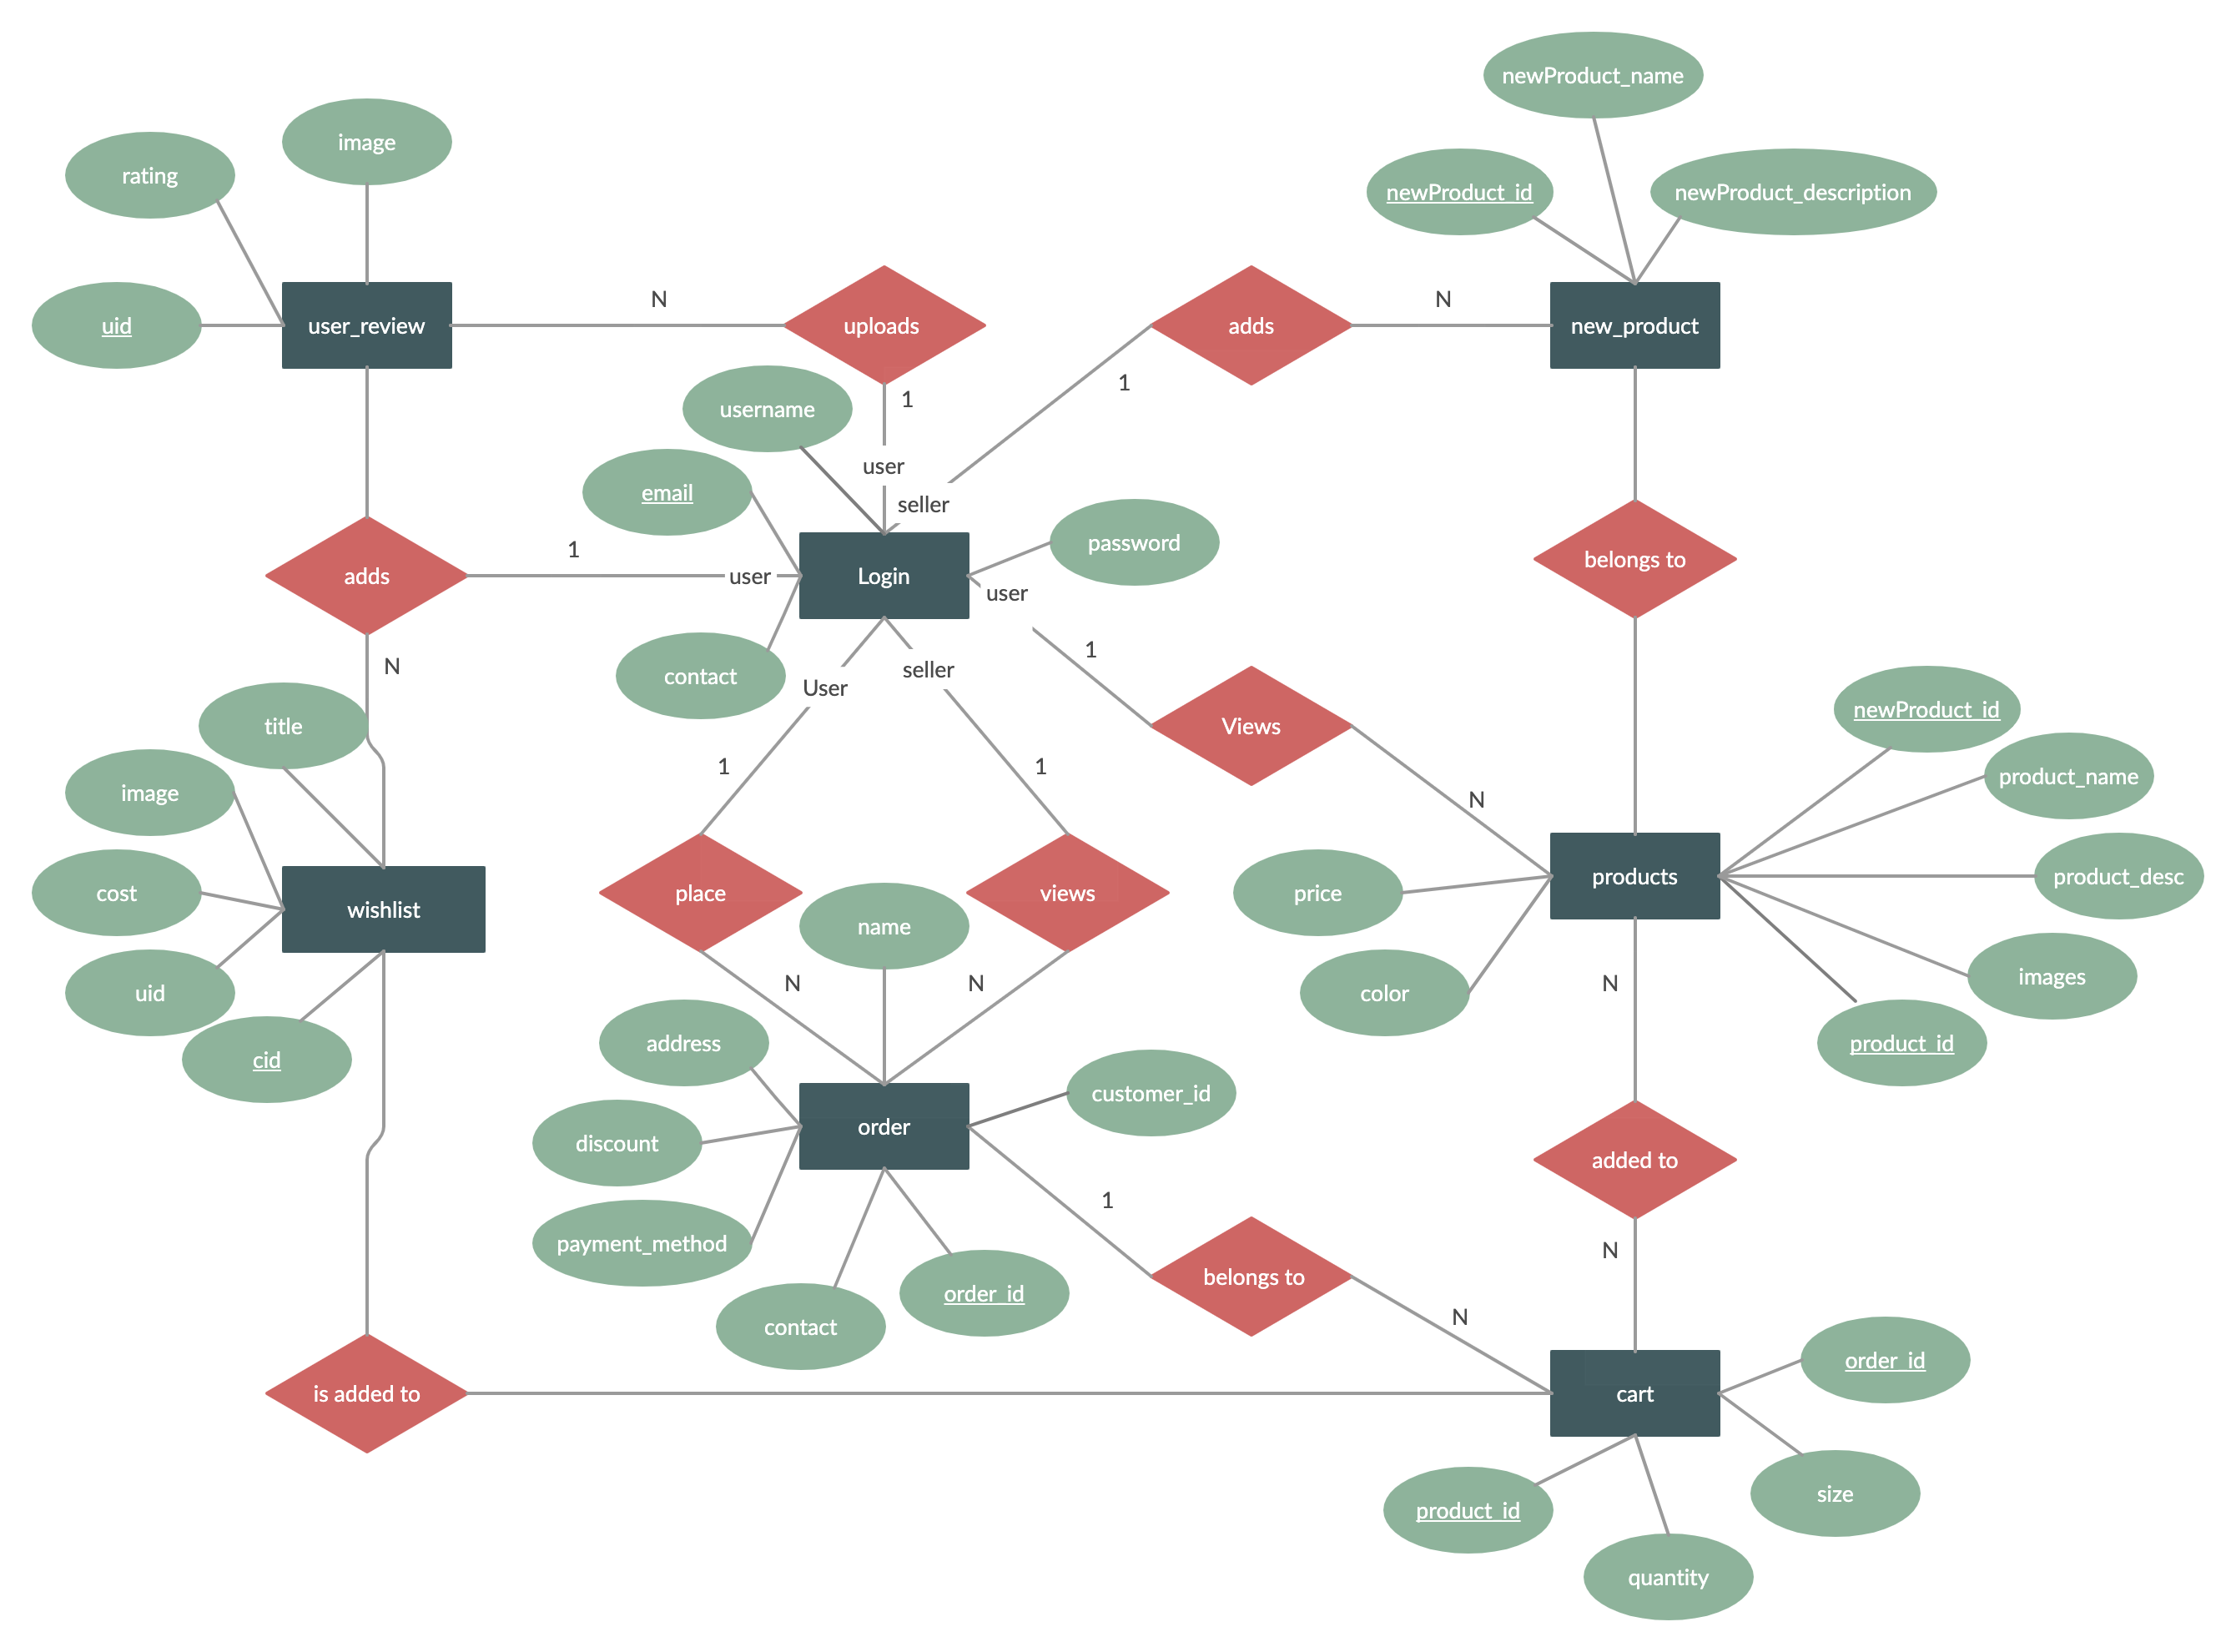
\includegraphics[width=\linewidth]{er.jpg}}
	\caption{ER Diagram.}
\end{figure} 
\begin{figure}[H]
	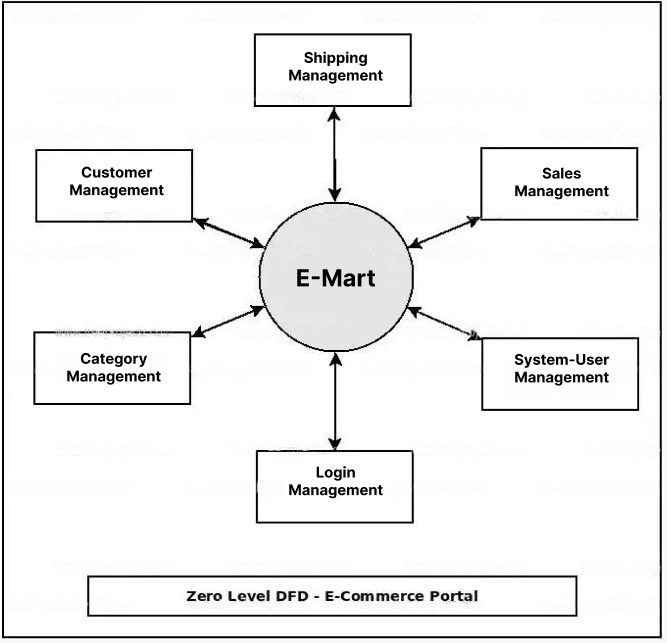
\includegraphics[width=\linewidth]{dfdl0.jpeg}
	\caption{Data Flow Diagram Level 0.}
\end{figure}
\begin{figure}[H]
	\fbox{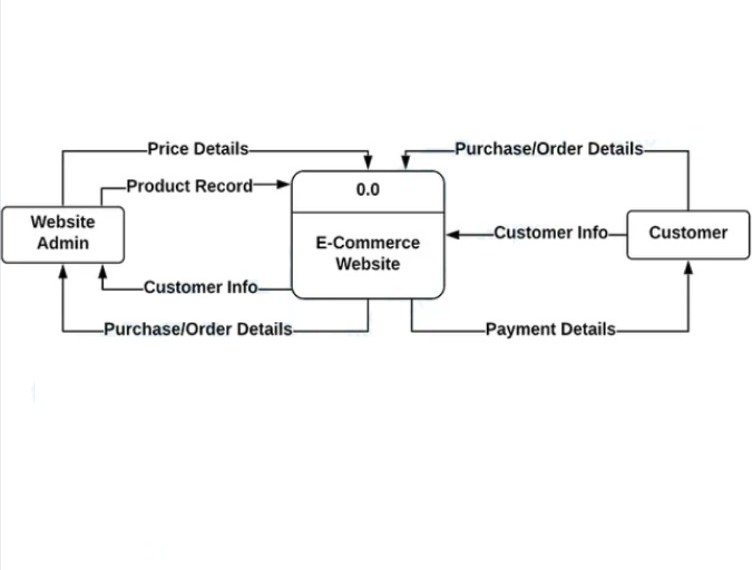
\includegraphics[width=\linewidth]{dfdl1.jpeg}}
	\caption{Data Flow Diagram Level 1.}
\end{figure}
\begin{figure}[H]
	\fbox{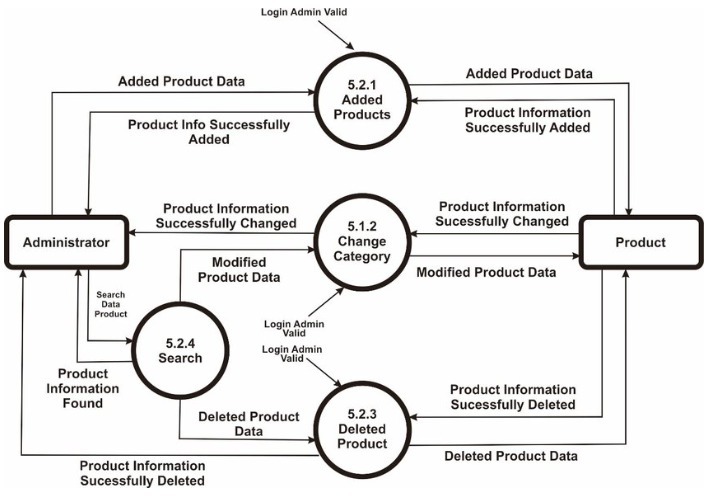
\includegraphics[width=\linewidth]{dfdl2.jpeg}}
	\caption{Data Flow Diagram Level 2 (Administrator).}
\end{figure}
\begin{figure}[H]
	\fbox{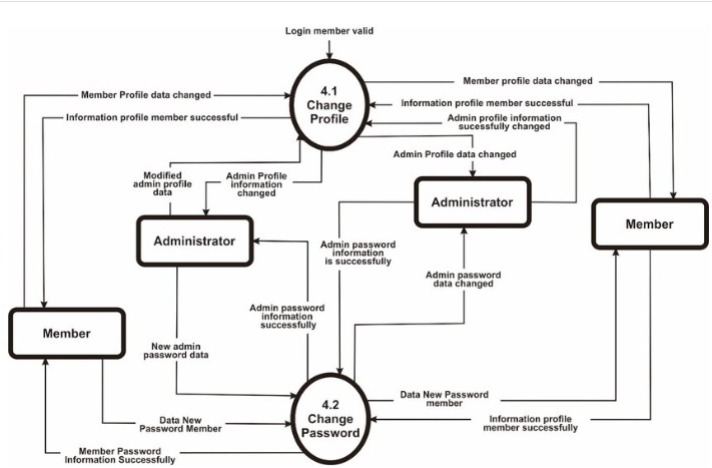
\includegraphics[width=\linewidth]{dfdl2-1.jpeg}}
	\caption{Data Flow Diagram Level 2 (Login).}
\end{figure}
\begin{figure}[H]
	\fbox{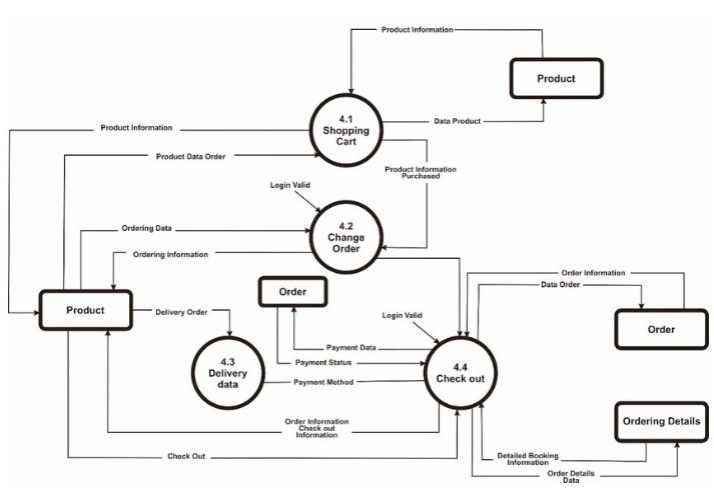
\includegraphics[width=\linewidth]{dfdl2-2.jpeg}}
	\caption{Data Flow Diagram Level 2 (User).}
\end{figure}
\section{Module Description}
The admin module deals with the login credentials of the administrator. The administrator has the power to and is the sole user that has the permissions to add  and manage exchanges and users. The admin module includes authorization with a username and password.
The add/edit exchange component through the admin module deals with the adding/editing of the exchange. In this component, the adding/editing of a particular exchange along with its requisite information can be done.
The add user component lets the administrator add each user with their passkey. \\
The user module deals with various components that a user can perform without login or authorization.
The add/edit holding component provides the user the power to add/edit a particular holding of a choice that can be both bitcoin and alt coin.
The view status component helps the user to view the status of the holdings along with the particular exchange that the holding was bought from.
The edit holding component can allow the user to edit the details of the exchange that was previously added by the user.\\
P2P Module deals with the lending component.
The lending component allows a user to borrow from another user various USD amounts that a particular user has for lending purposes.

\section{Hardware \& Software Requirements}
\textbf{HARDWARE REQUIREMENTS} \\
The hardware required for the development of this project is:\\
- RAM: 2GB \\
- Dual Core Processor \\
- Display \\
\\\textbf{SOFTWARE REQUIREMENTS}\\
- Python (Django) \\
- Javascript (React)\\
- MySQL and related services \\
- VS Code IDE \\
- Web Browser such as Chromium.\\

\section{Work Schedule}
The work schedule was done in an organized manner. The project took a duration of 10 days. Initial days comprised of designing and visualizing the project concept. The tables and their descriptions were also produced. Later days comprised of developing the project. Further days consisted of testing the project. Fine tuning the project along with design modifications were done on the final days of the project.

\chapter{Screenshots}
\begin{figure}[H]
	\fbox{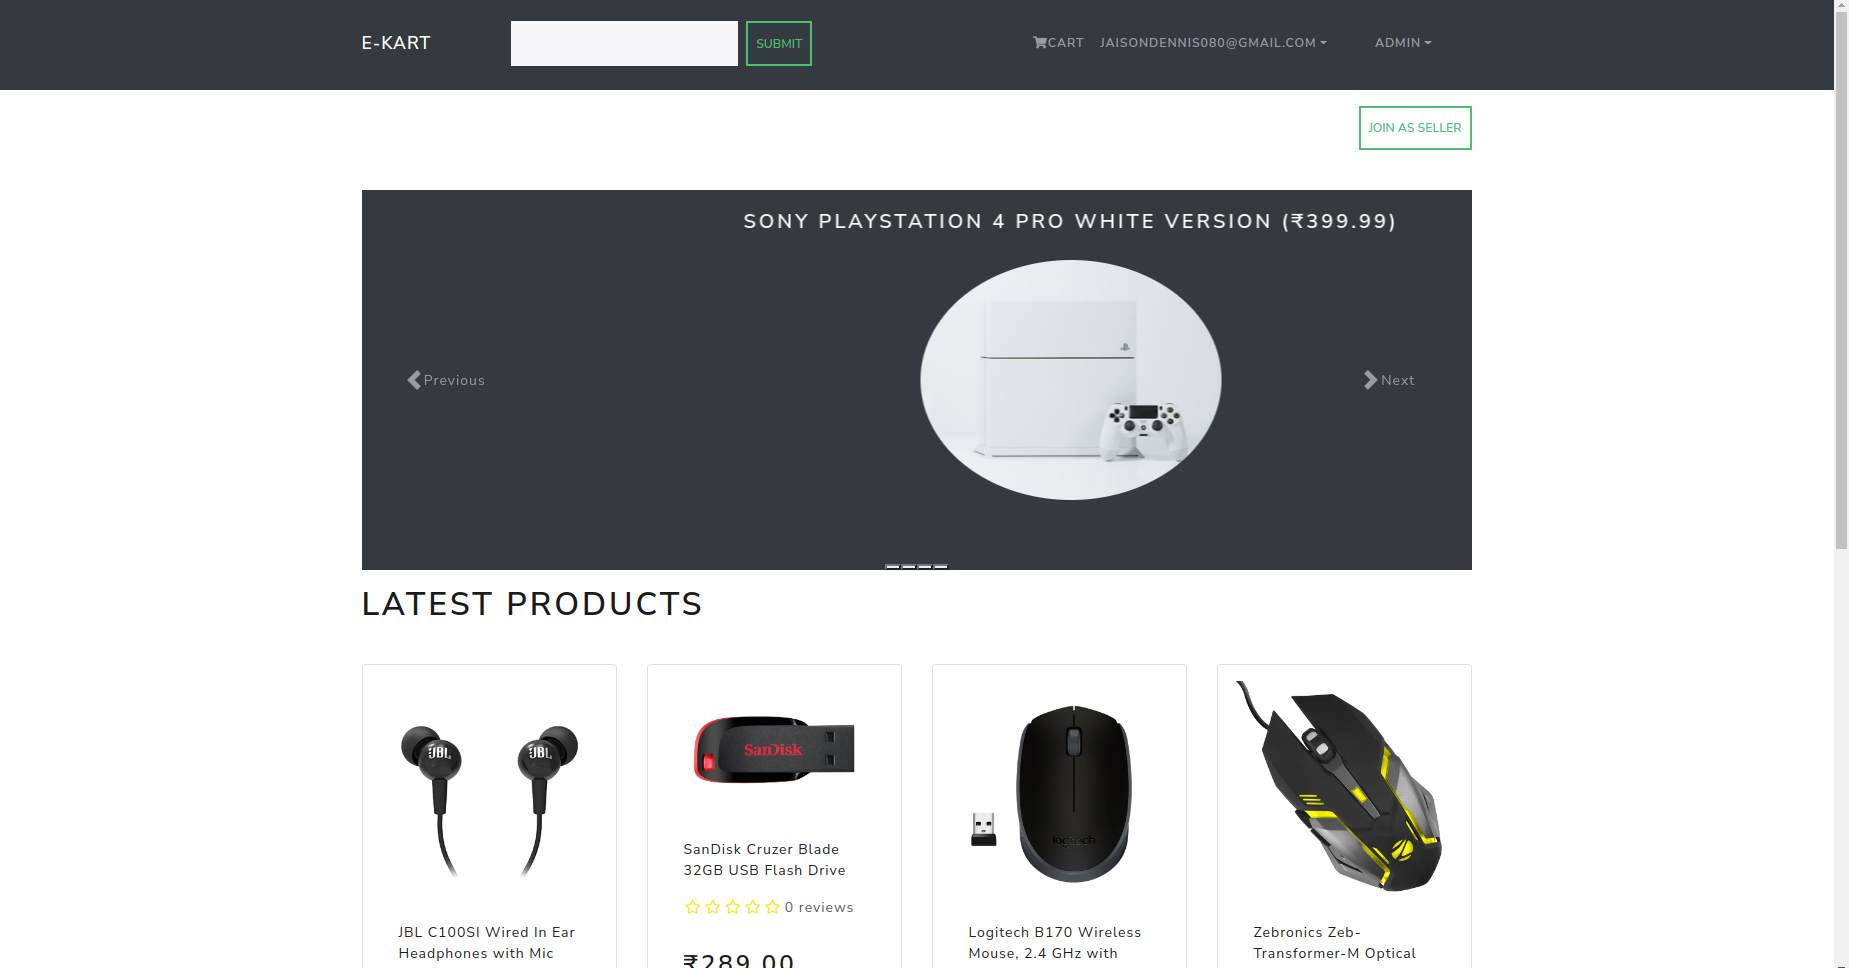
\includegraphics[width=\linewidth]{home.png}}
	\caption{Home Screen}
	\label{fig:erd}
\end{figure} 
\begin{figure}[H]
	\fbox{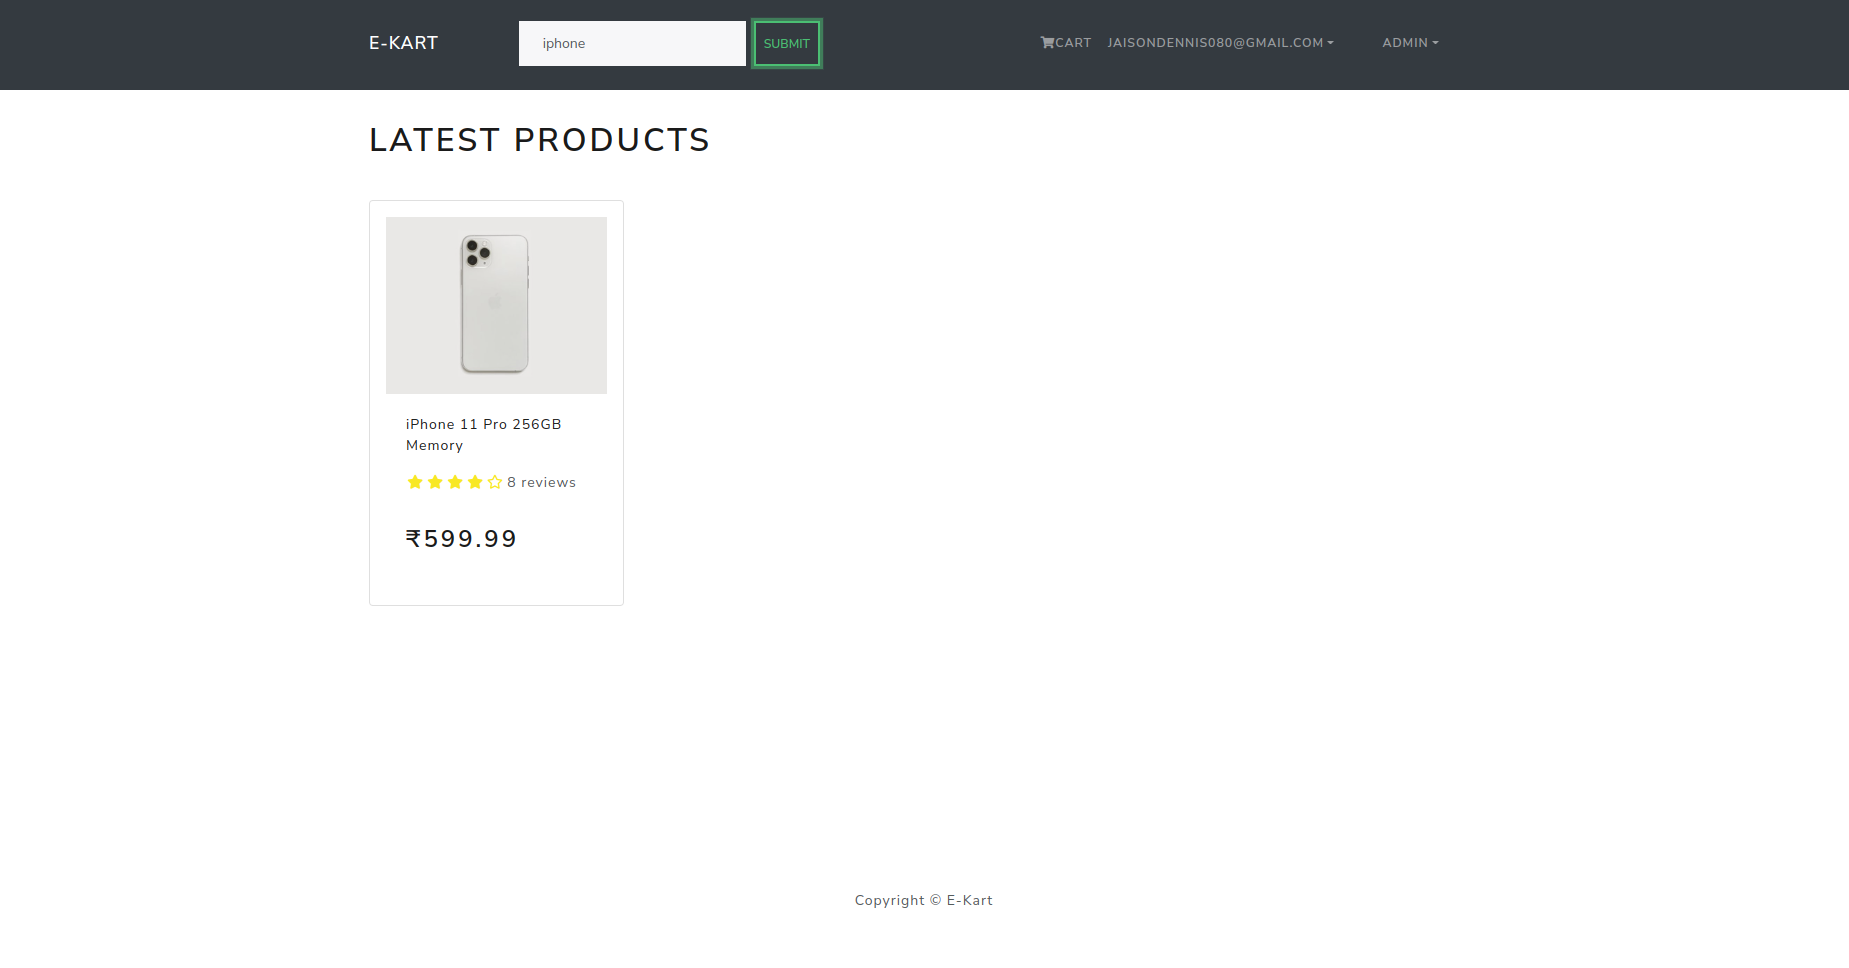
\includegraphics[width=\linewidth]{search.png}}
	\caption{Search Products}
	\label{fig:dfd}
\end{figure}
\begin{figure}[H]
	\fbox{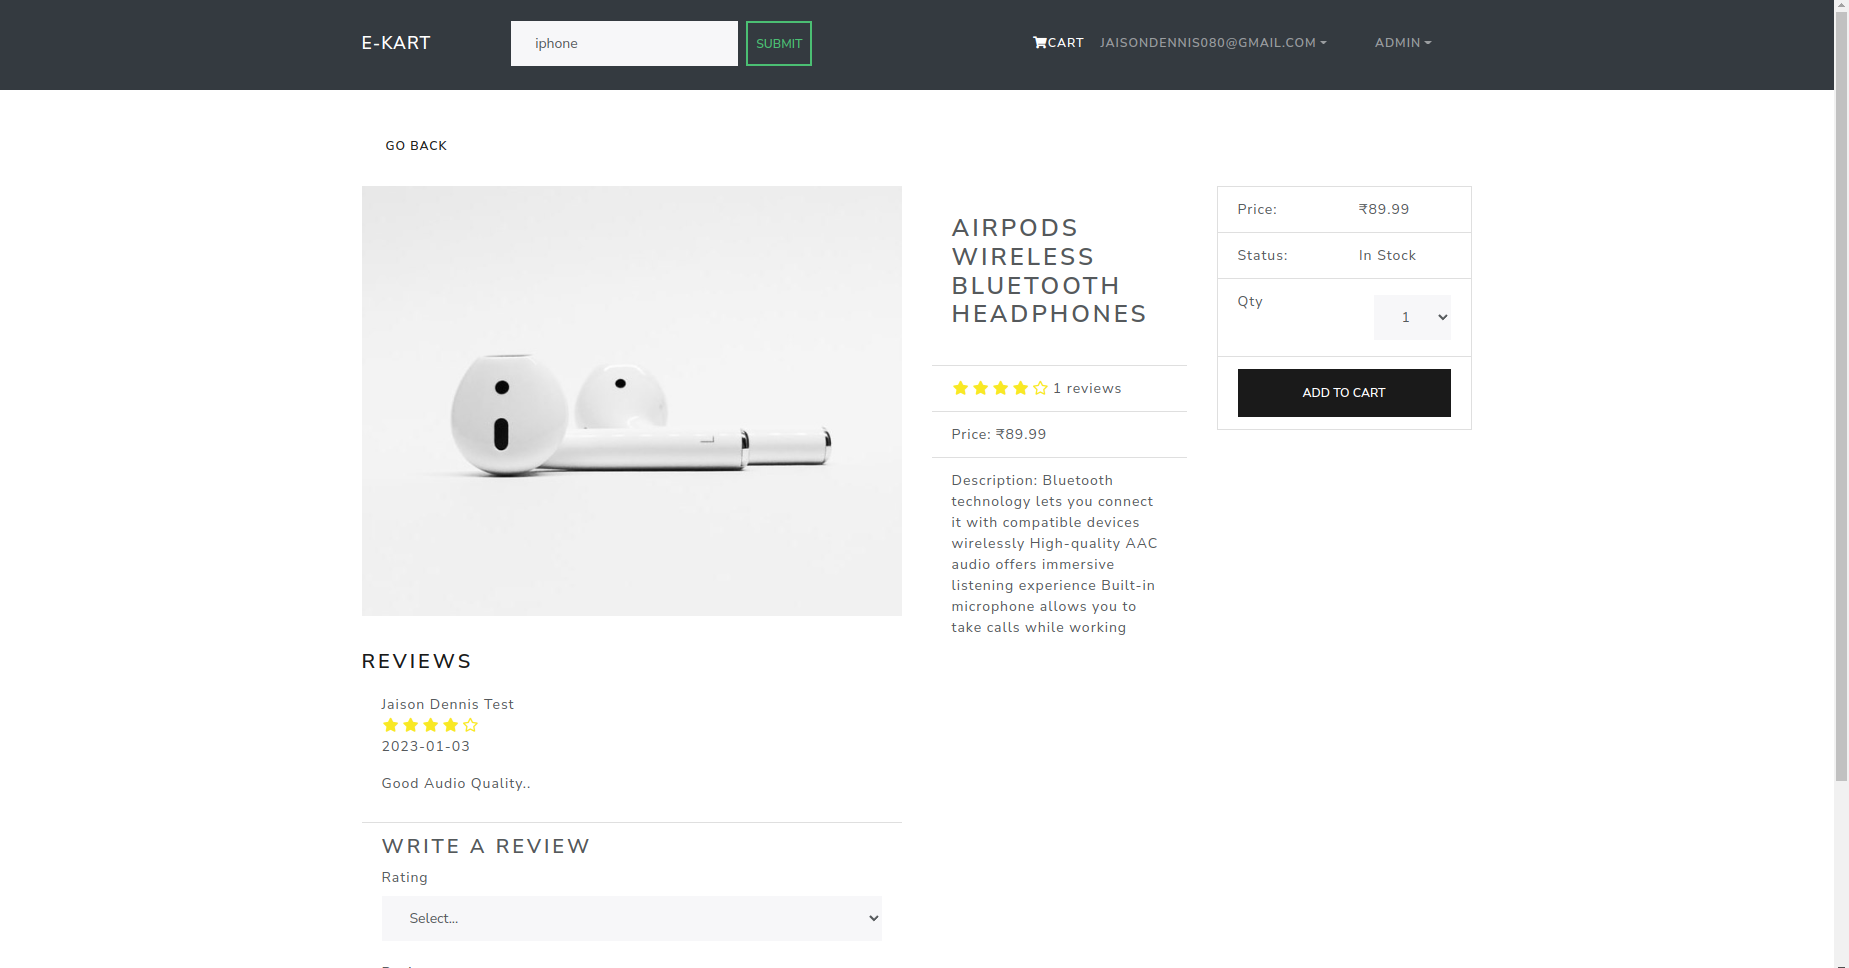
\includegraphics[width=\linewidth]{description.png}}
	\caption{Product Description}
	\label{fig:dfd2}
\end{figure}
\begin{figure}[H]
	\fbox{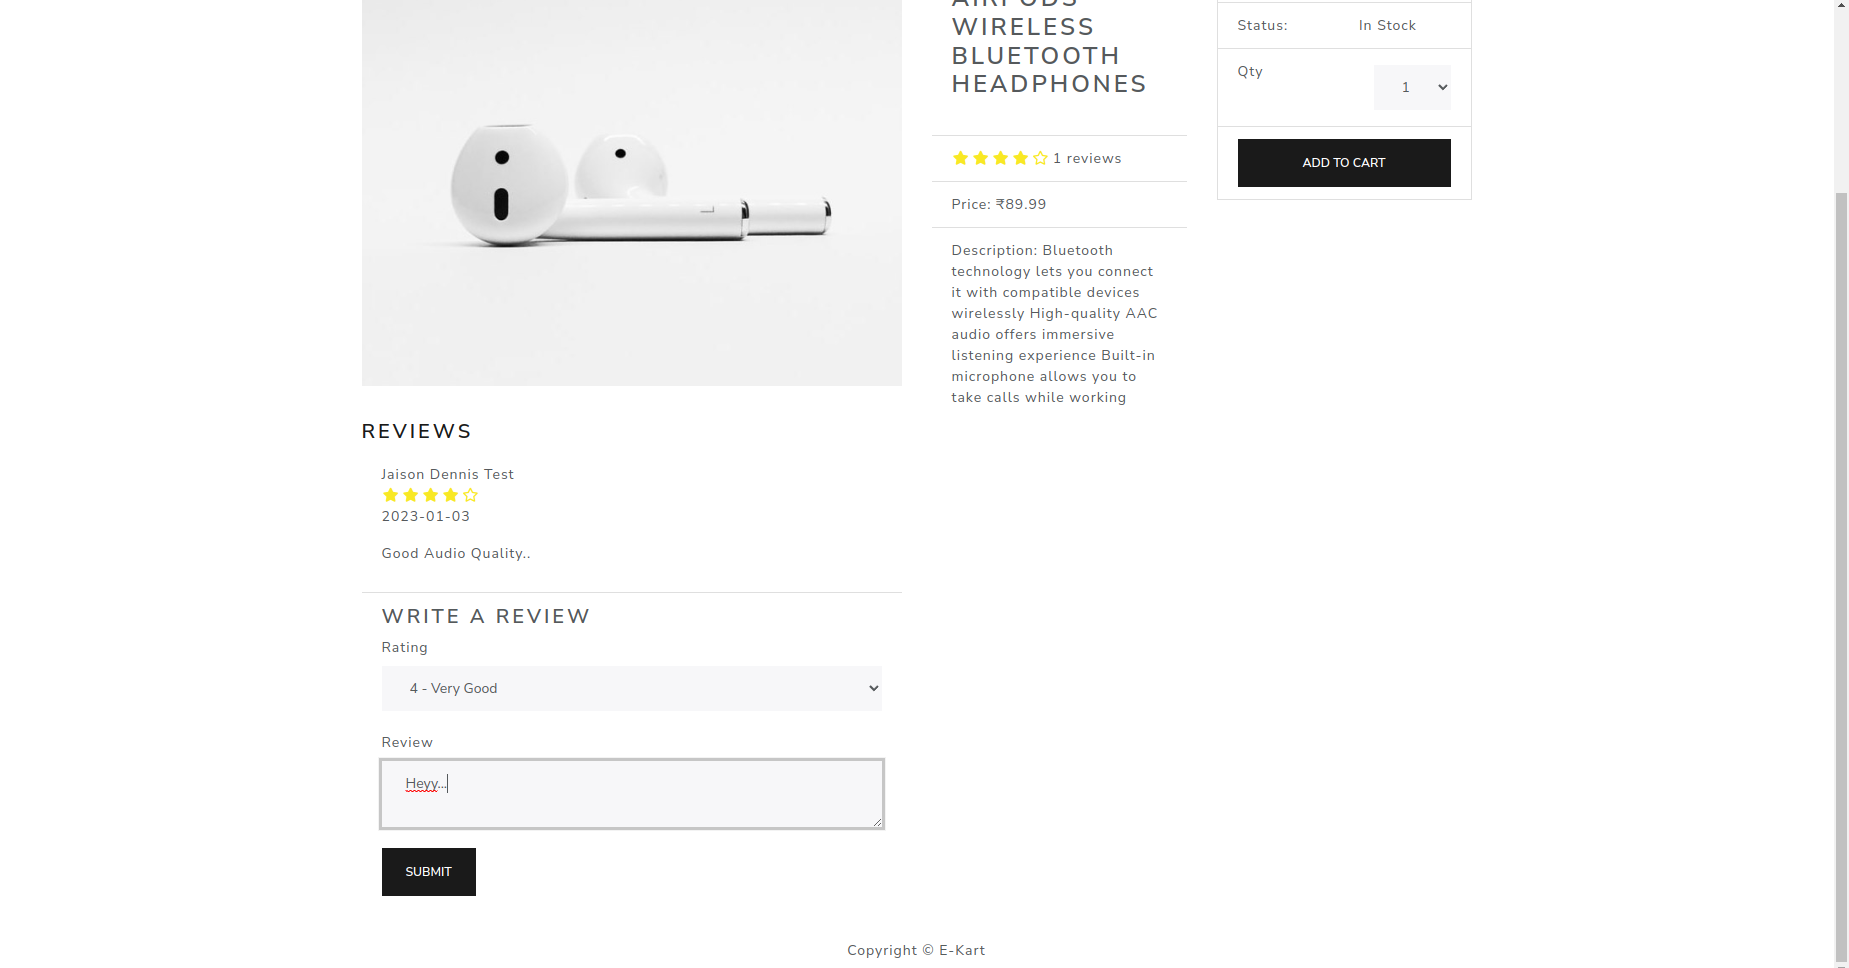
\includegraphics[width=\linewidth]{review.png}}
	\caption{Reviews}
	\label{fig:dfd3}
\end{figure}
\begin{figure}[H]
	\fbox{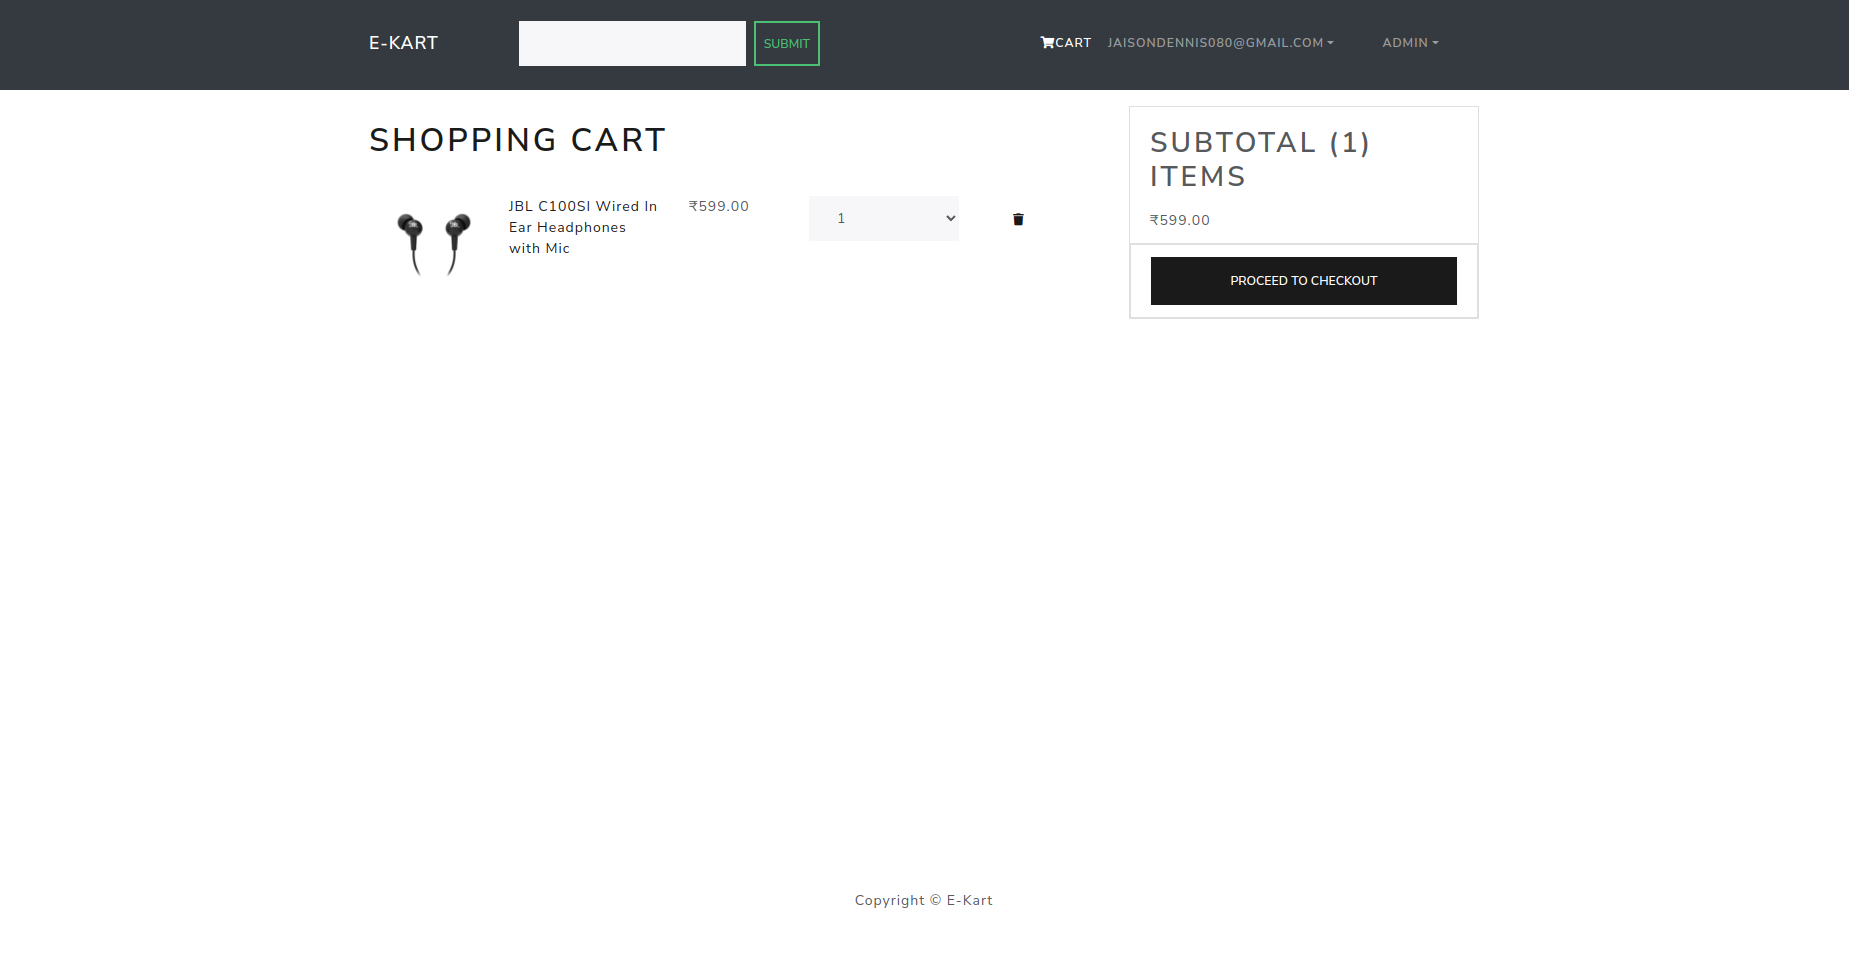
\includegraphics[width=\linewidth]{cart.png}}
	\caption{Shopping Cart}
	\label{fig:s5}
\end{figure}
\begin{figure}[H]
	\fbox{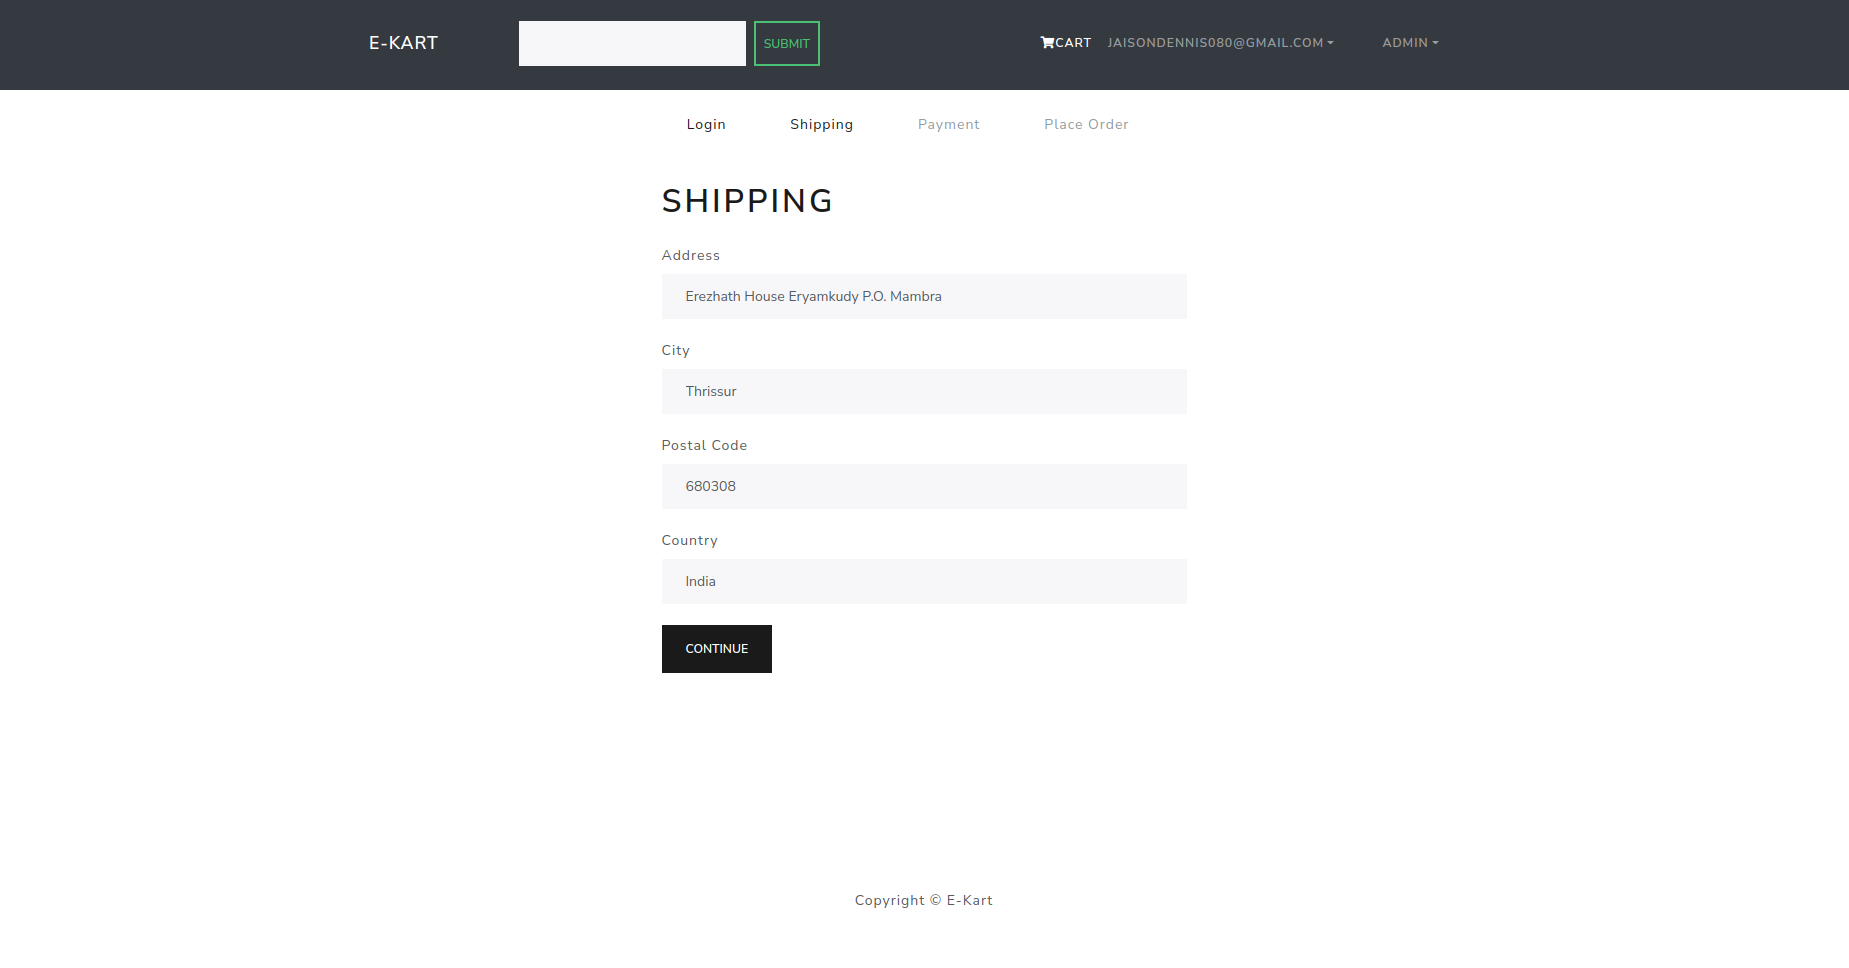
\includegraphics[width=\linewidth]{shipping.png}}
	\caption{Shipping Details}
	\label{fig:s6}
\end{figure} 
\begin{figure}[H]
	\fbox{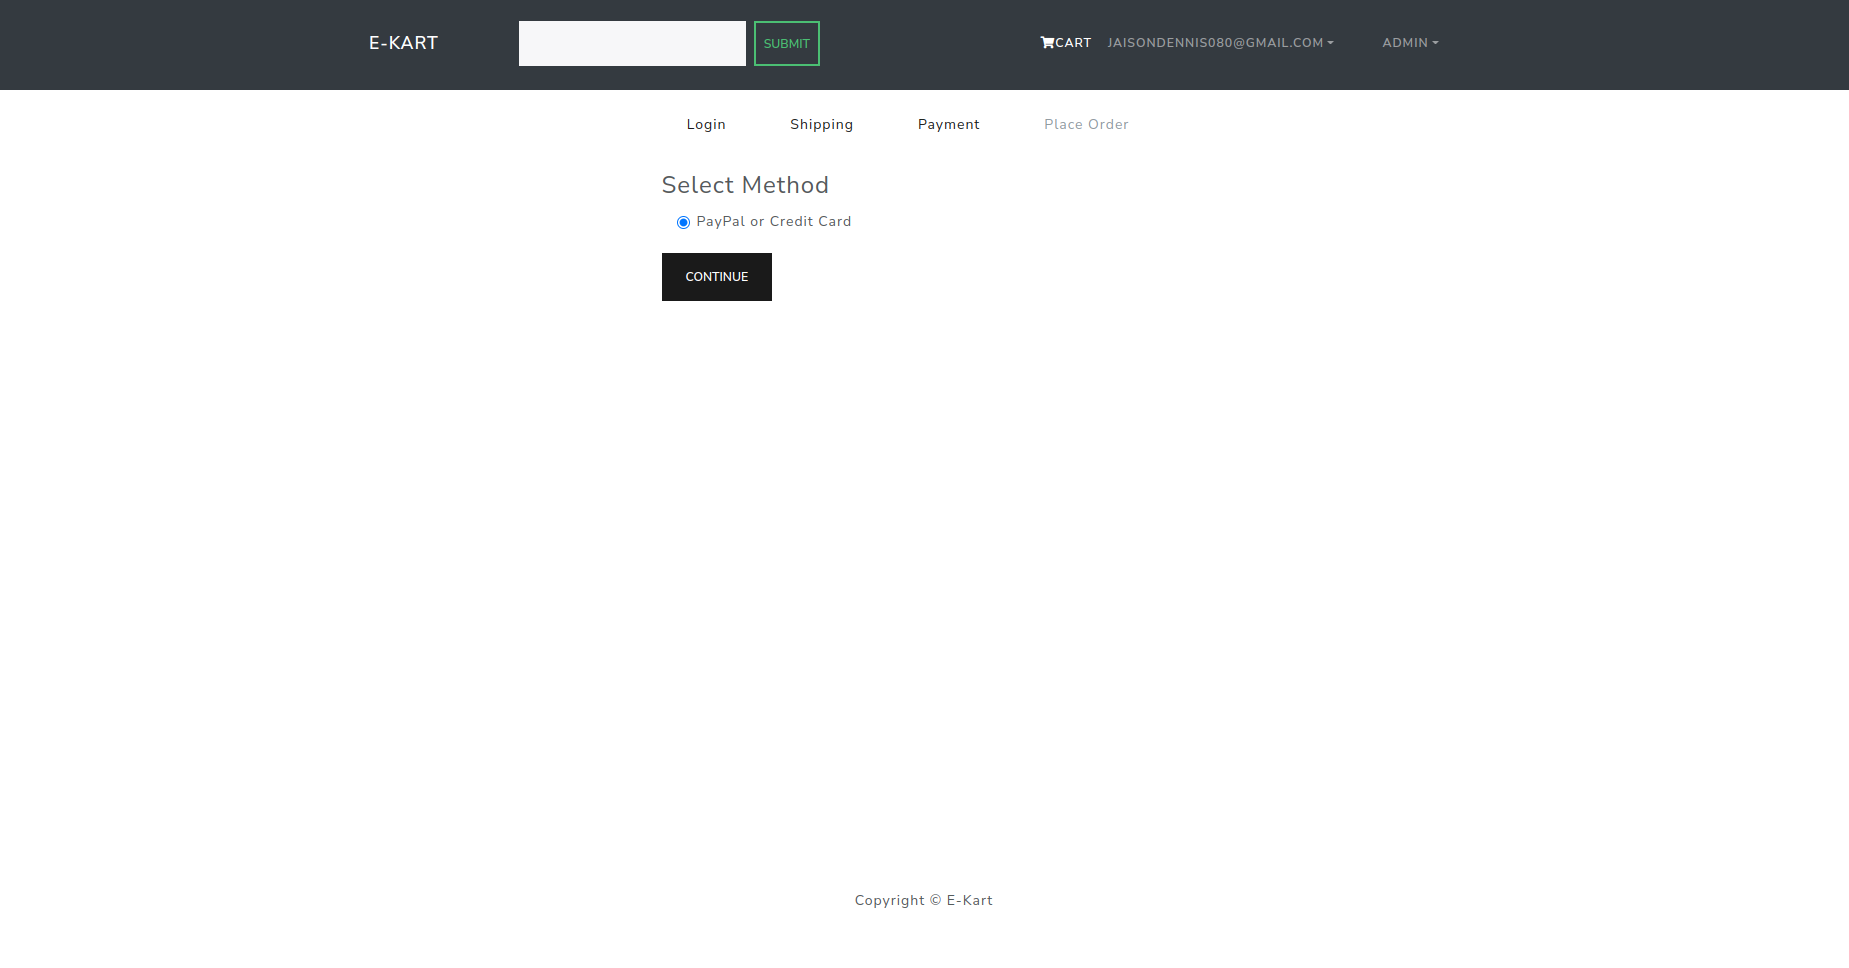
\includegraphics[width=\linewidth]{payment.png}}
	\caption{Payment Method}
	\label{fig:s7}
\end{figure}
\begin{figure}[H]
	\fbox{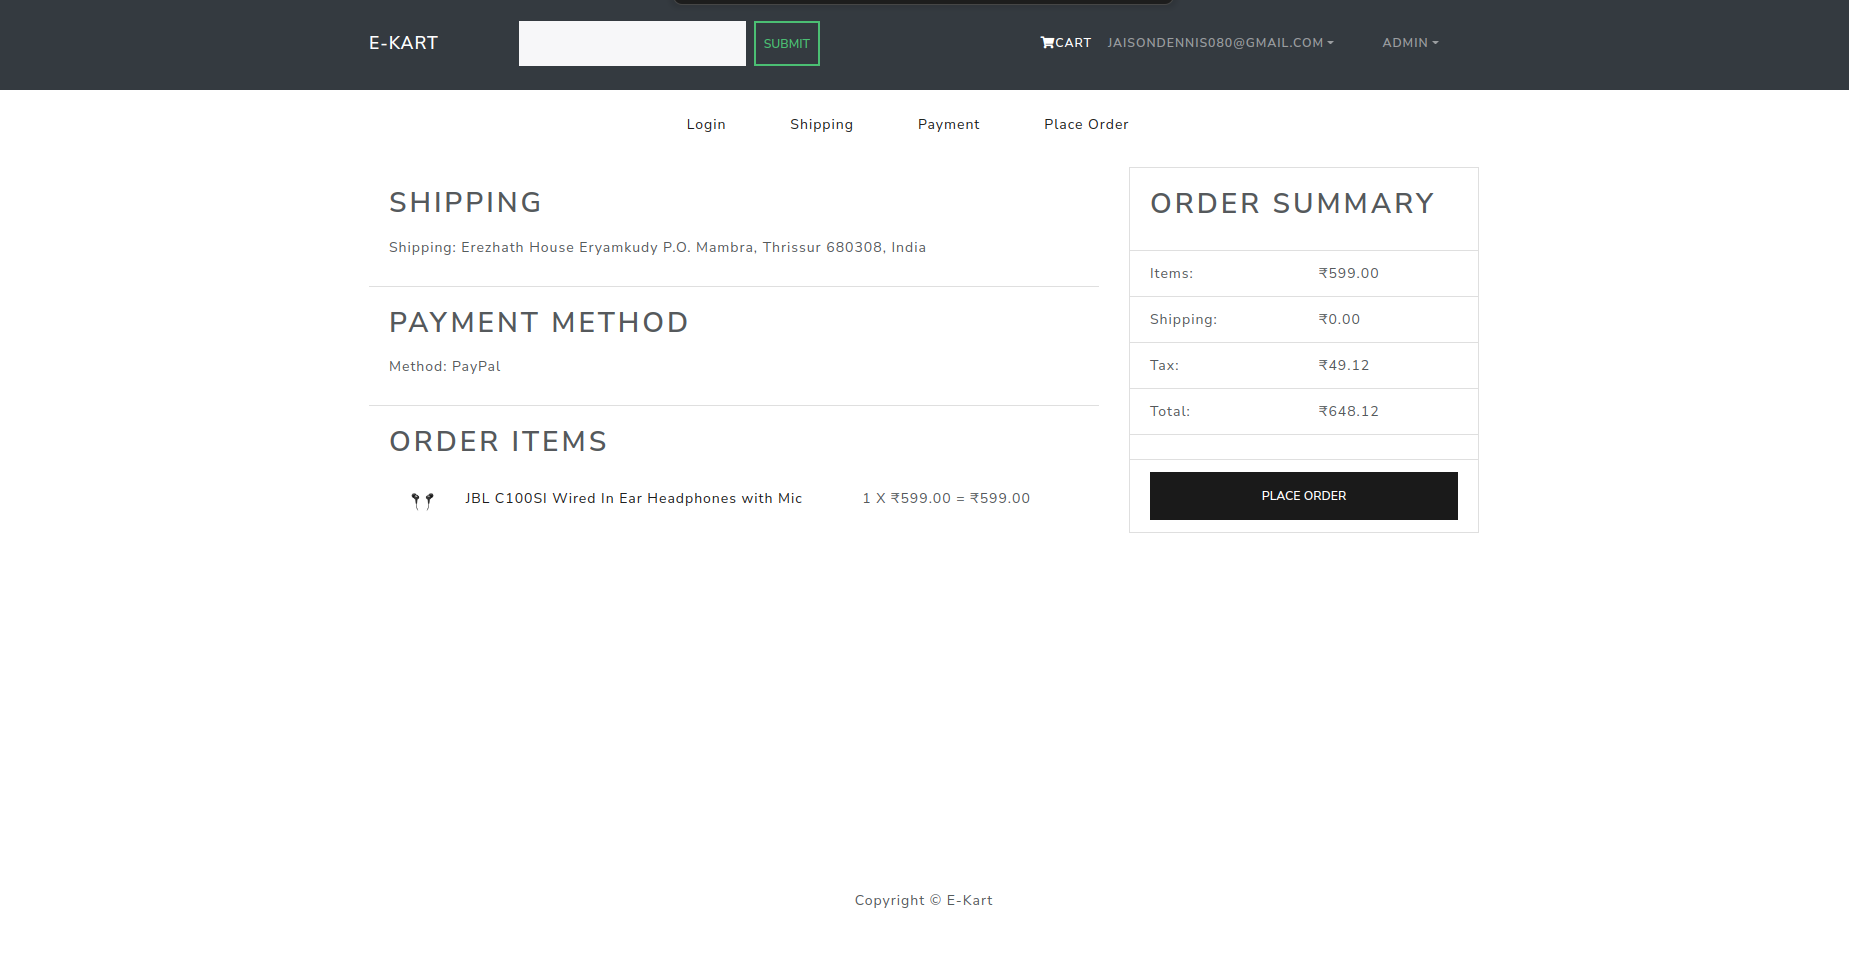
\includegraphics[width=\linewidth]{confirm.png}}
	\caption{Confirm Order}
	\label{fig:s8}
\end{figure}
\begin{figure}[H]
	\fbox{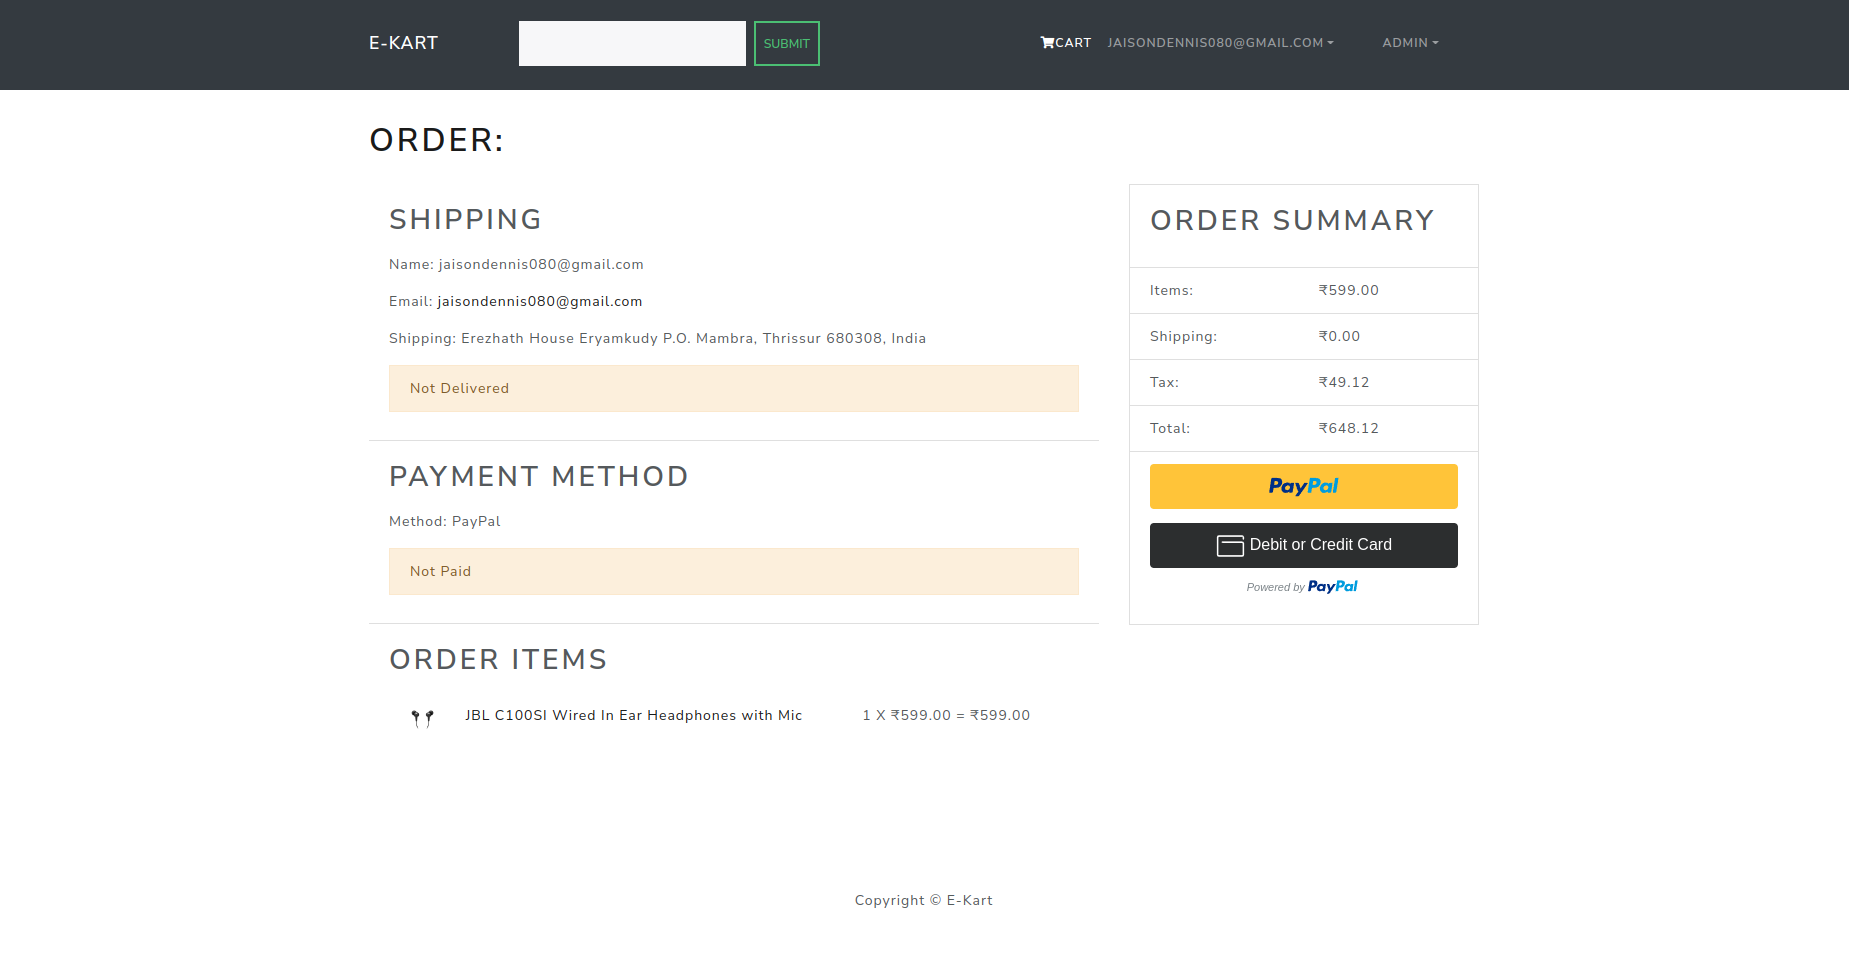
\includegraphics[width=\linewidth]{status.png}}
	\caption{Order Status}
	\label{fig:s9}
\end{figure}
\begin{figure}[H]
	\fbox{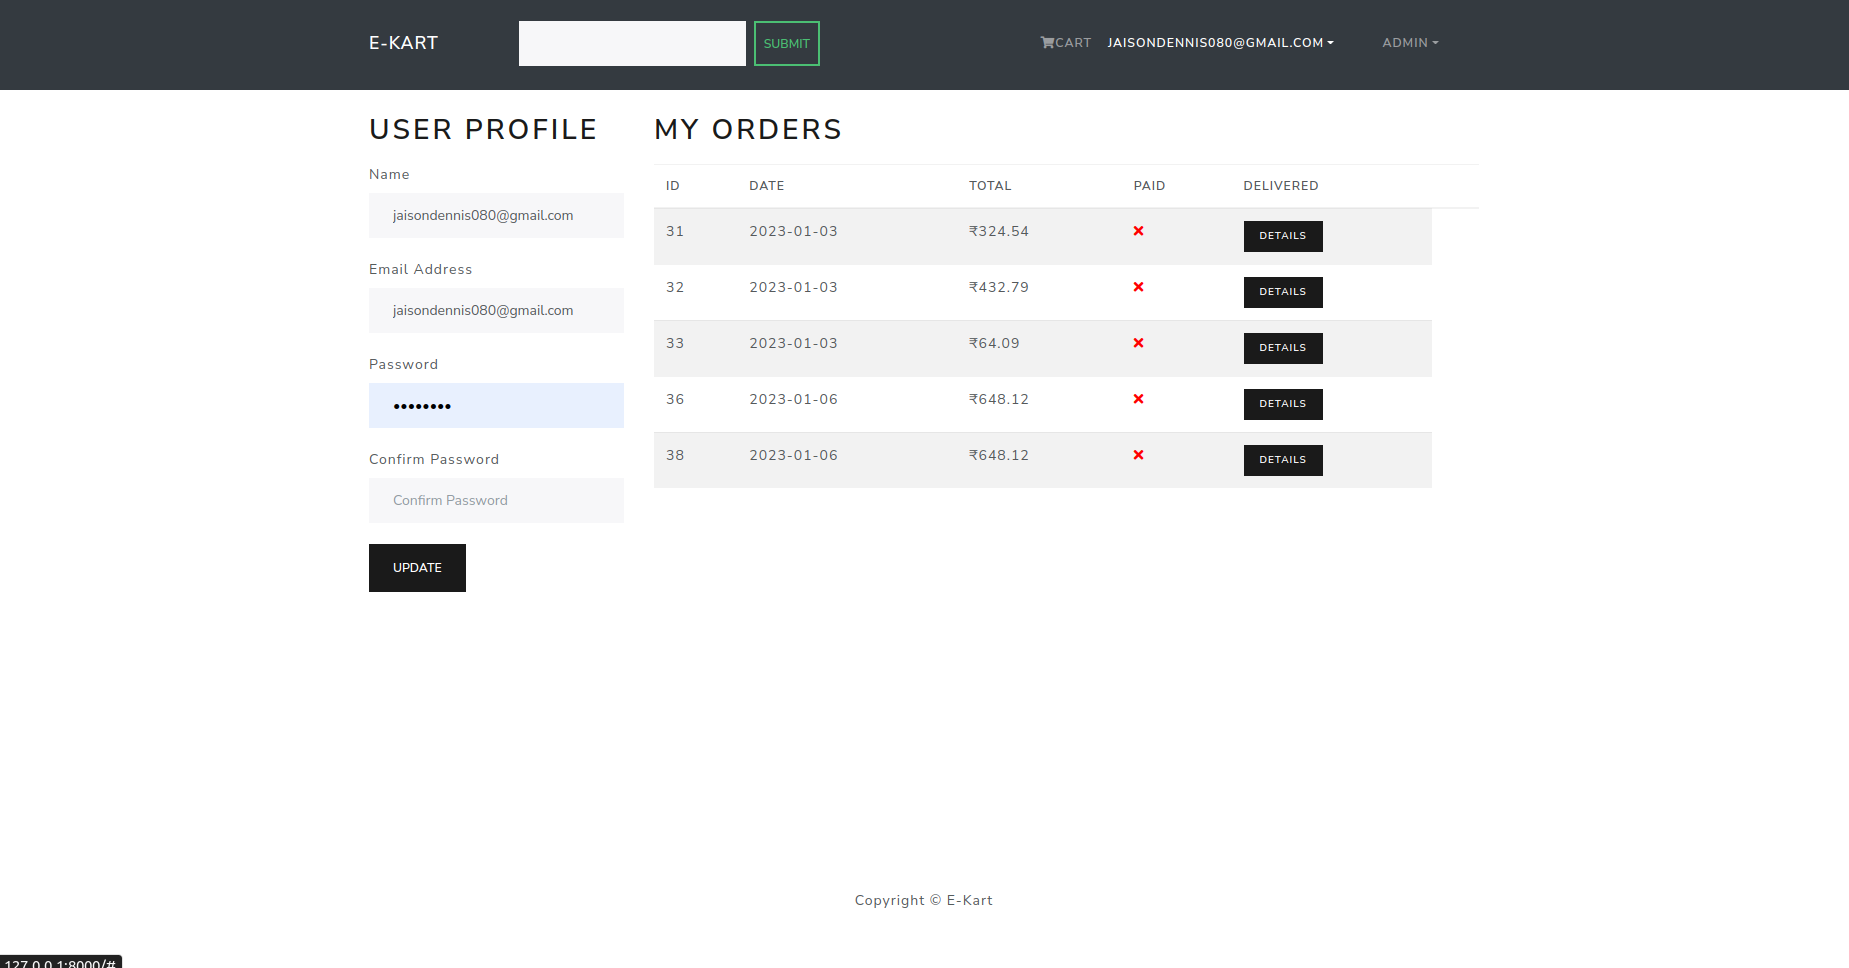
\includegraphics[width=\linewidth]{profile.png}}
	\caption{User Profile}
\end{figure}
\begin{figure}[H]
	\fbox{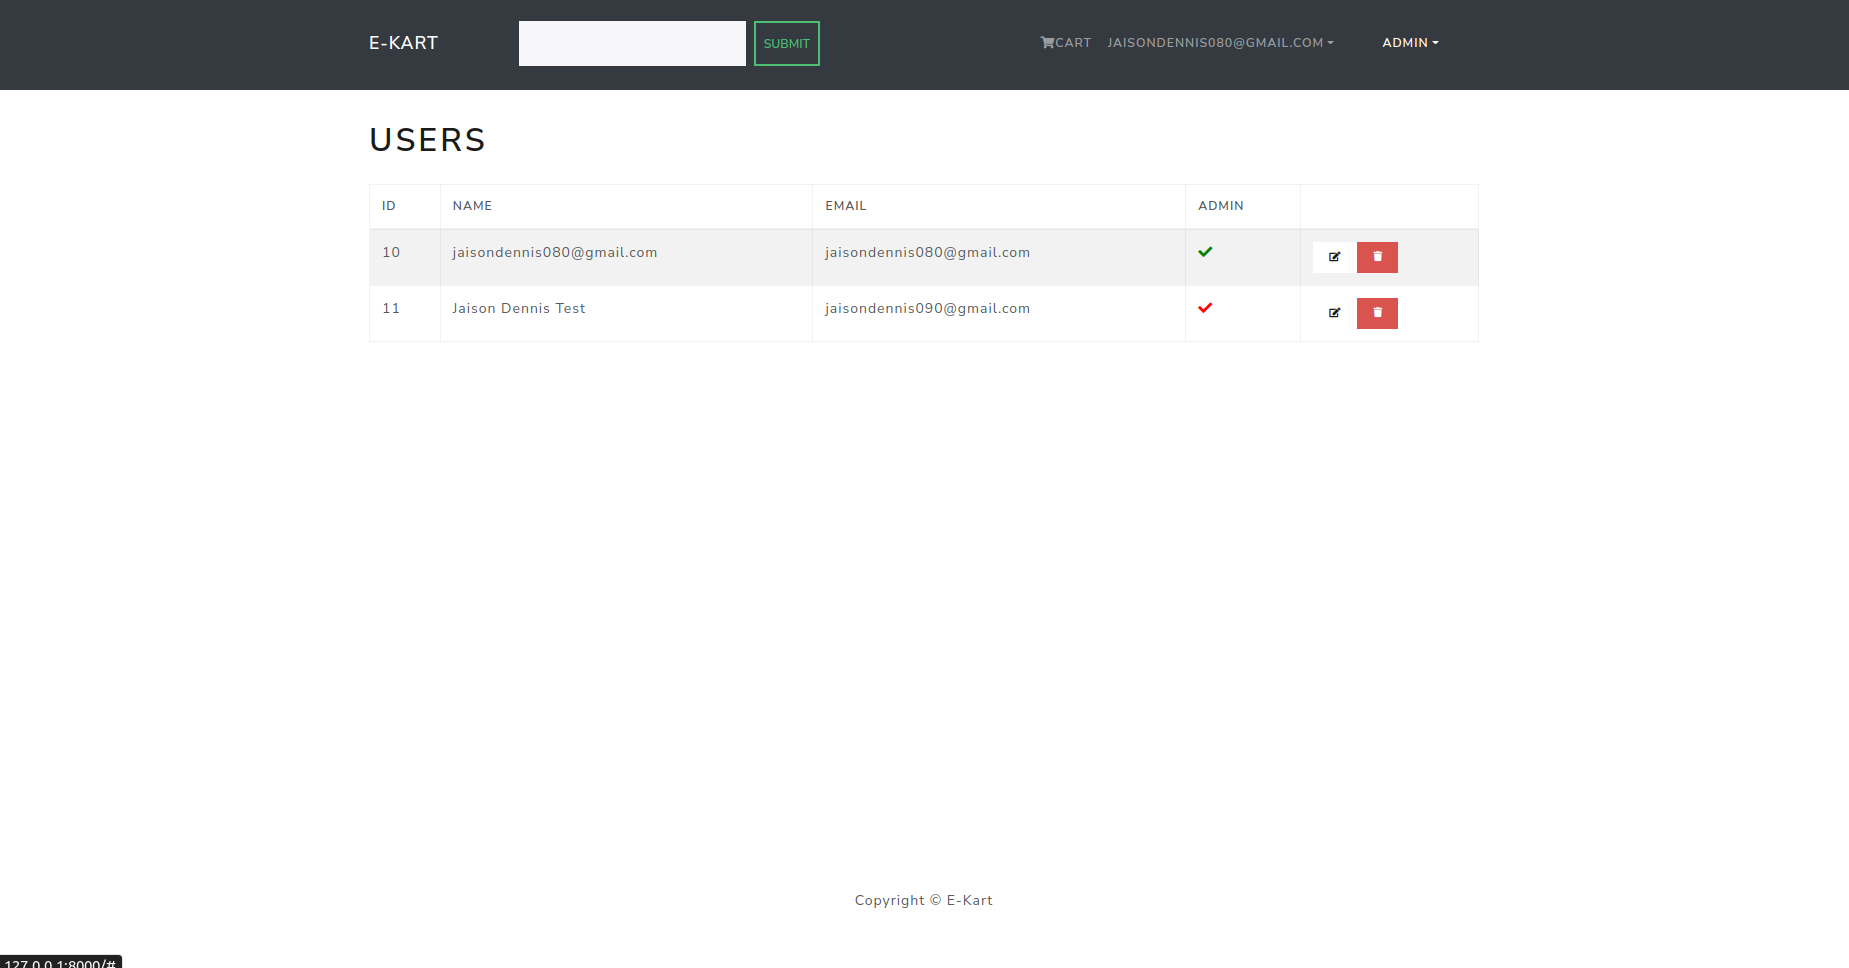
\includegraphics[width=\linewidth]{users.png}}
	\caption{View Users}
\end{figure}
\begin{figure}[H]
	\fbox{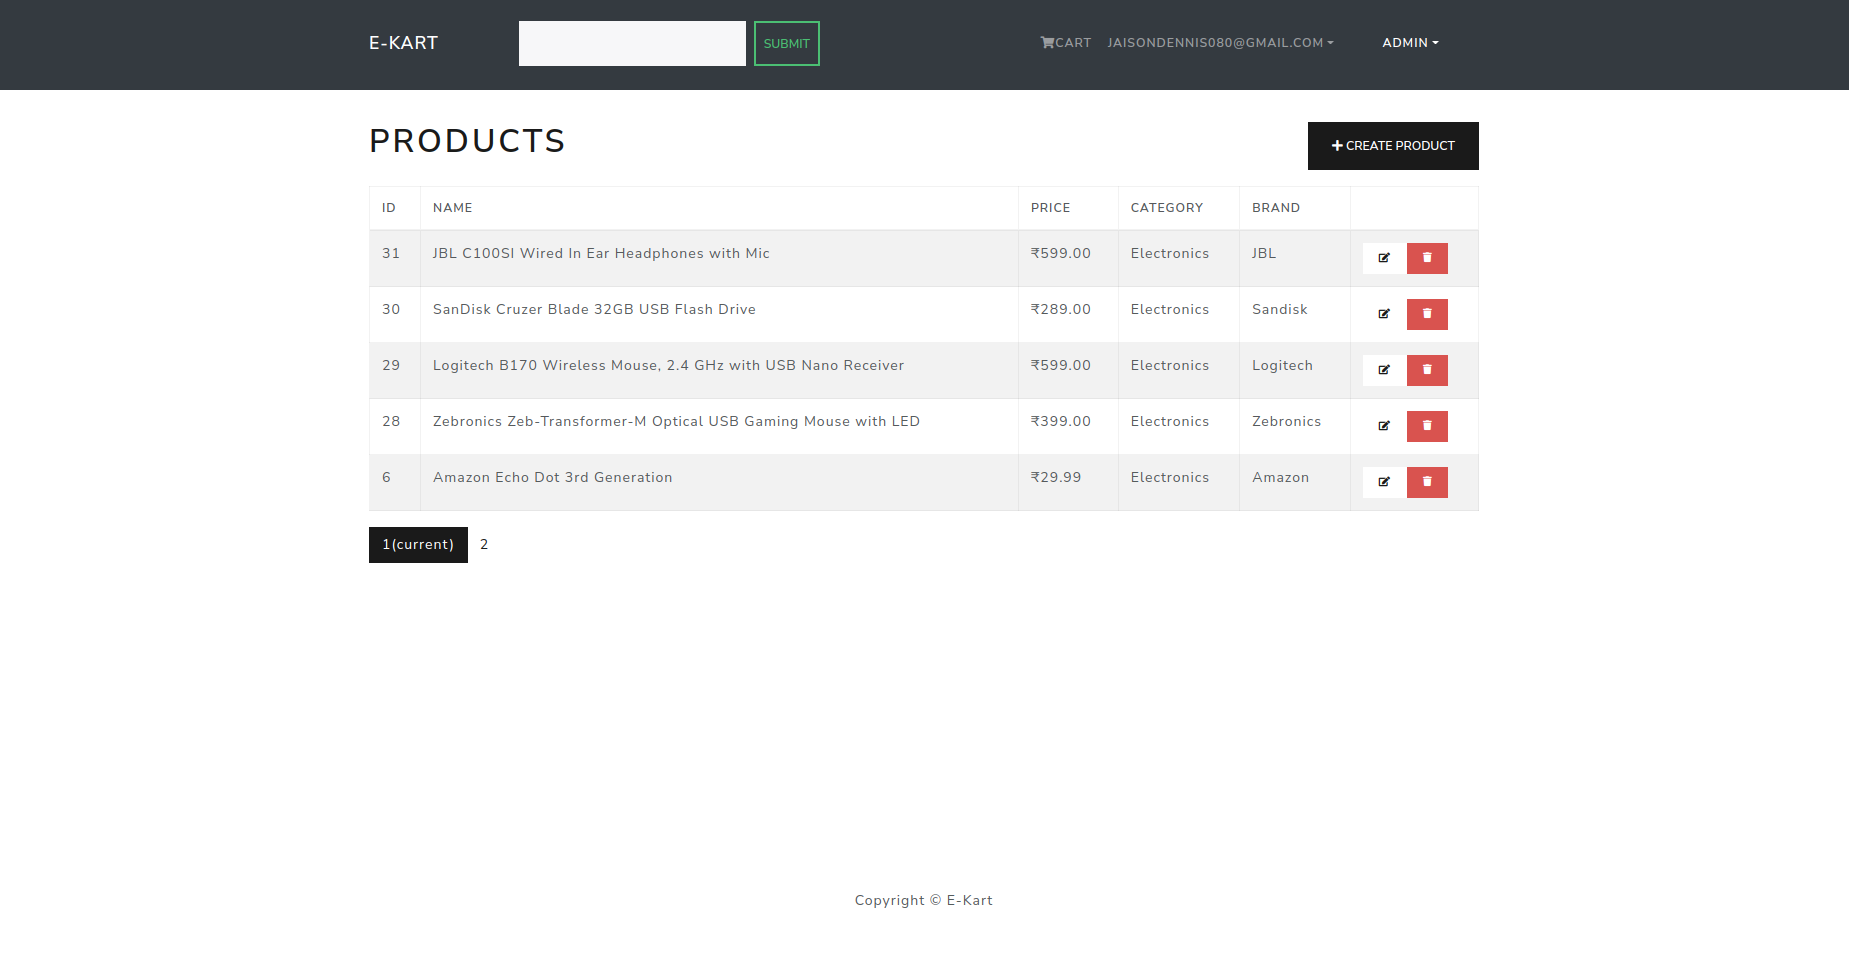
\includegraphics[width=\linewidth]{products.png}}
	\caption{View Products}
\end{figure}
\begin{figure}[H]
	\fbox{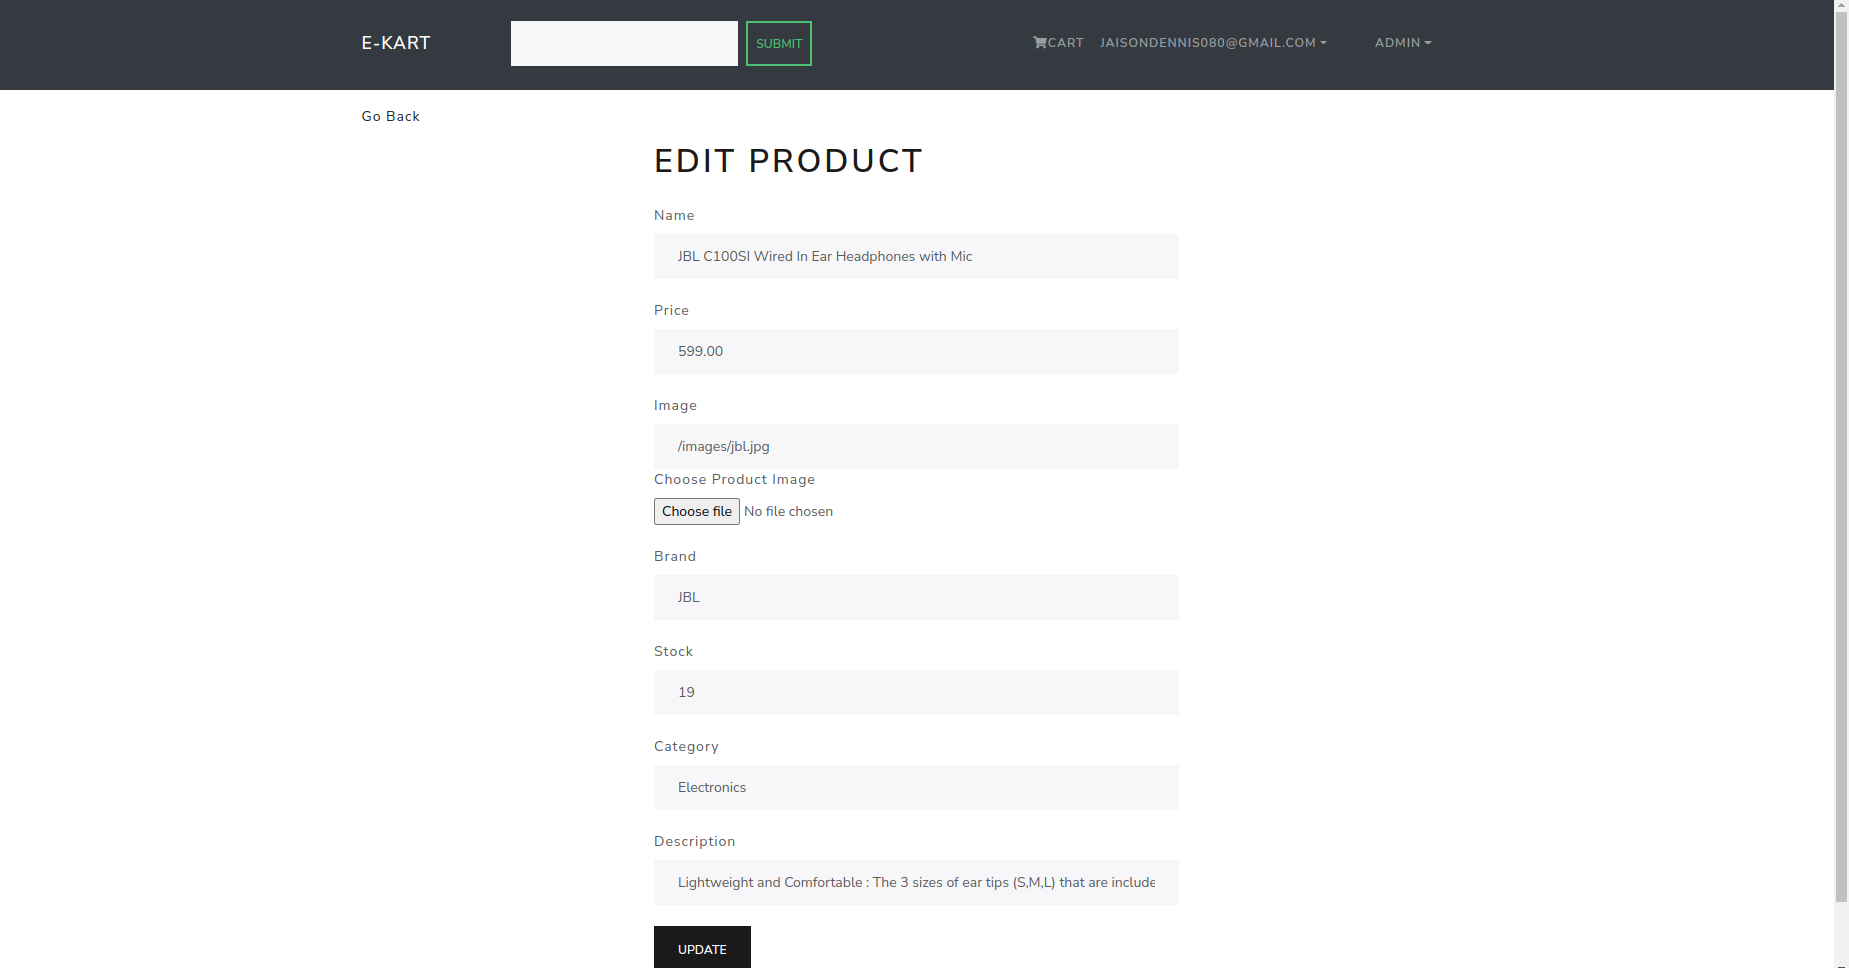
\includegraphics[width=\linewidth]{editproduct.png}}
	\caption{Edit Product}
\end{figure}
\begin{figure}[H]
	\fbox{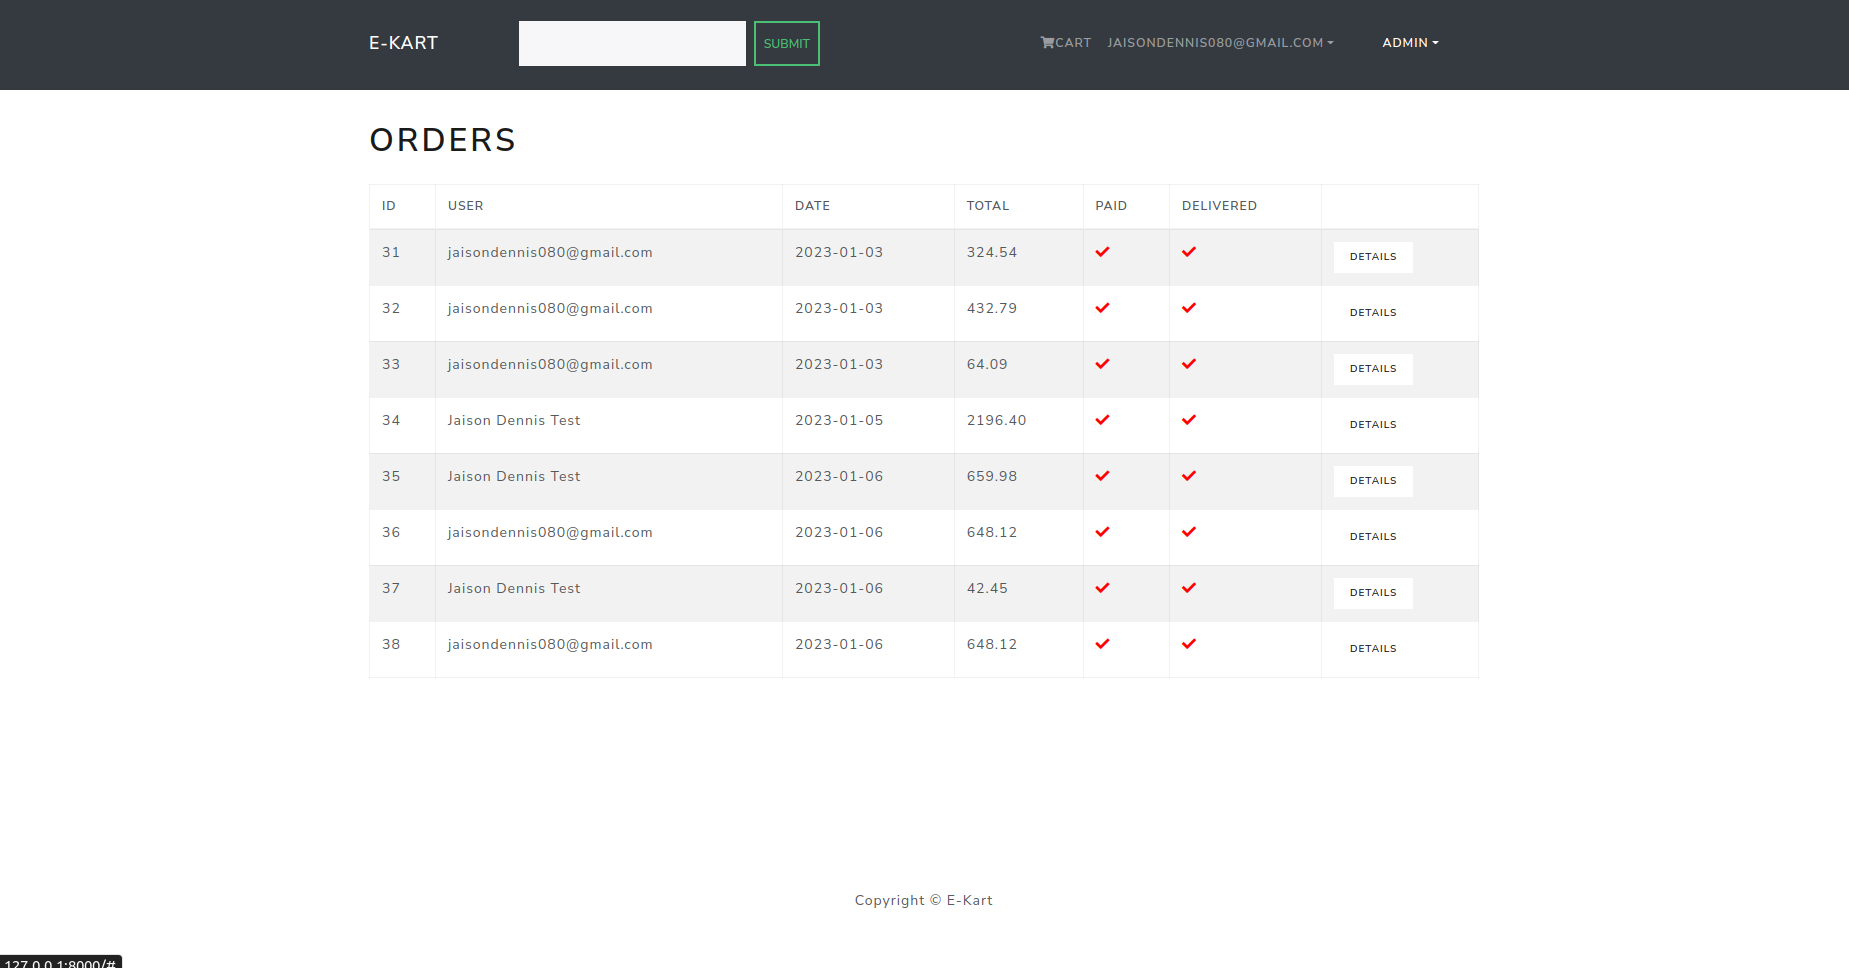
\includegraphics[width=\linewidth]{orders.png}}
	\caption{View Orders}
\end{figure}
 \chapter{Conclusion}
 E-Mart ecommerce software with the functional modules was successfully developed and a secured
 digitalized and user-friendly system for the easy add, delete and editing of ecommerce products also featuring provisons to order and purchase products by uesrs.
 Manually maintained operations where computerized so that the user can rely on their memory
 less. Thus the system created to overcome the problems effectively without any corrupted data or
 information.It is found to be bug-free as per the testing standards that are implemented. And by
 specification, untraced errors will be concentrated in the coming versions, which is planned to be
 developed in the near future.The user finally has all that they need to have an
 purchase, add, track order and delete ecommerce products thus providing users a pleasant and seamless experience.
 \label {con}


 

   
%\begin{thebibliography}{999}
%\addcontentsline{toc}{chapter}{References}
%\bibitem{sas}  M Sasikumar, Dinesh Shikkare, P Ravi Prakash: 
%	Introduction to Parallel Processing: First Edition, PHI, New Delhi, 2000
%\bibitem{raj} V Rajaraman. S SivaRama Murthy: 
%	Parallel Computer Architecture and Programming: PHI, New Delhi, 2000
%\bibitem{dav} David HM Spector: Building Linux Clusters: O'Reilly \& associates, 
%CA, USA, 2000
%\bibitem{bar} Thomas C Bartee: Introduction to Computer Science: Third Edition, 
%McGraw-Hill, New York, 1975
%\bibitem{nlb} http://www.netlib.org/pvm3/: PVM software source
%
%\end{thebibliography}
\begin{thebibliography}{999}
\addcontentsline{toc}{chapter}{References}

\bibitem{re1} https://www.builder.ai/
\bibitem{re2} https://amazon.in/
\bibitem{re3} 

\end{thebibliography}


\end{document}
